%% Based on techreport.tex template as sent by Erik Burger on 2023-11-20
%% 
%% Karlsruhe Institute of Technology
%% Institute for Program Structures and Data Organization
%% Chair for Software Design and Quality (SDQ)
%%
%% Dr.-Ing. Erik Burger
%% burger@kit.edu
%%
%% See https://sdq.kastel.kit.edu/wiki/Dokumentvorlagen
%%
%% Version 1.0, 2023-11-20

%% Available page modes: oneside, twoside
%% Available languages: english, ngerman
%% Available modes: draft, final (see README)
\documentclass[oneside, ngerman]{sdqtechreport}

%% ---------------------------------
%% | Information about the document |
%% ---------------------------------

%% Name of the group and authors
\author{Paul Buda, Martin Scheuermann, Stephan Schneider, \\
Simon Schütz und Nils Seibert}

%% Title (and possibly subtitle) of the thesis
\title{Pflichtenheft}

\subtitle{zur Android-App Neptune}

%% You can put a logo in the ``logos'' directory and include it here
%% instead of the SDQ logo
% \grouplogo{myfile}
%% Alternatively, you can disable the group logo
% \nogrouplogo

\date{01.12.2023}

%% For example texts -- please remove in the final version
\usepackage{blindtext}

%% ====================================
%% ====================================
%% ||                                ||
%% || Beginning of the main document ||
%% ||                                ||
%% ====================================
%% ====================================
\begin{document}

%% Set PDF metadata
\setpdf

%% Set the title
\maketitle

%% ------------------------
%% |   Table of Contents  |
%% ------------------------
\tableofcontents

%% -----------------
%% |   Main part   |
%% -----------------
\cleardoublepage

%% -------------------
%% | Example content |
%% -------------------

\chapter{Einleitung}
\label{chap:Einleitung}

\section{Einführung}
\label{sec:Einleitung:Einführung}
Musik spielt im Leben vieler Menschen eine enorm wichtige Rolle. Insbesondere bei Partys und Zusammenkünften mit Freunden ist eine gute Musikauswahl essentiell für eine gute Stimmung unter den Anwesenden. Aber auch der umgekehrte Fall ist vielen sicherlich gut bekannt – gefällt die abgespielte Musik den Anwesenden nicht, so kann dies die Stimmung erheblich trüben.

Während die Musikauswahl bei größeren und insbesondere bei kommerziellen Veranstaltungen üblicherweise durch das Engagement professionell arbeitender DJs übernommen wird, obliegt sie bei kleineren Veranstaltungen in der Regel dem Gastgeber. Aufgrund der weiten Verbreitung von Musikstreaming-Diensten werden dann häufig vorkonfigurierte Playlists abgespielt - was es schwierig macht, die musikalischen Vorlieben der Anwesenden zu erfüllen.

Nahezu alle heute gängigen Musikstreaming-Anbieter versuchen bereits mit proprietären Lösungen, dem entgegenzuwirken. In der Anwendung jedoch sind die eigens von den Anbietern angebotenen Lösungen häufig nicht praktikabel. Die Ursachen hierfür sind divers, so setzen sie beispielsweise häufig voraus, dass alle Teilnehmer über ein bestehendes Abonnement beim entsprechenden Anbieter verfügen. Zudem gibt es häufig keine oder nur schlecht umgesetzte Abstimmungsfunktionen.

Ziel des Projekts „Neptune“ ist es, eine praktikable Lösung für die eingangs beschriebene Problematik zu entwickeln. Hierzu soll im Rahmen des Moduls „Praxis der Softwareentwicklung“ eine Android-App entwickelt werden, mithilfe derer die Anwesenden bei einer Party oder einem vergleichbaren Event gemeinsam über die abgespielte Musik entscheiden können. 





\section{Anwendungsbereiche}
\label{sec:Einleitung:Anwendungsbereich}

Das Ziel von Neptune ist es, die Musikauswahl bei privaten Veranstaltungen, wie zum Beispiel studentische WG- und Wohnheimpartys, einfacher und gerechter zu gestalten.
Die Android-App Neptune bietet Gruppen die Möglichkeit jeden an der Musikauswahl zu beteiligen und über die Abspielreihenfolge demokratisch abzustimmen. Durch die Integration mit einem Audio-Streaming-Dienst wie Spotify kann Neptune automatisch die am besten bewerteten Tracks abspielen. Damit ist es möglich Songwünsche von Gästen zu erfüllen, ohne einen aktiven ''DJ''  der die Wünsche entgegen nimmt und sie manuell in die Warteschlange hinzufügt.

Bei der Erstellung einer Session kann der Gastgeber die verfügbaren Tracks nach Belieben auf verschiedene Genres/Artists oder eine Playlist beschränken. Nach Auswahl des Modus kann der Gastgeber die Gäste einladen, sich an der Musikauswahl zu beteiligen, indem er einen sechsstelligen Zahlencode oder einen Link weitergibt. Die Gäste können dann in der App Tracks in die Vorschlagsliste hinzufügen und mit dem Verteilen von Upvotes Tracks in der Liste nach oben voten und sie somit schneller zum Abspielen bringen. Der Host hat durch eine Kontrollansicht einen Überblick über die Queue, sowie die Vorschlagsliste in Neptune. Er kann in dieser Ansicht Tracks in die Queue hinzufügen und entfernen, sowie Tracks aus der Vorschlagsliste sperren, dadurch hat der Host weiterhin die volle Kontrolle über die Musikauswahl. Zusätzlich kann er durch die Einstellung
eines Cooldowns verhindern, dass diesselben Tracks mehrmals mit geringen Abstand gespielt werden.

Eine vollständige Beschreibung der Anwendungsfälle sind  den \hyperlink{Anwendungsfaelle}{Use Case Diagrammen (A 4)} zu entnehmen   


\section{Zielgruppe}
\label{sec:Einleitung:Zielgruppe}

Die primäre Zielgruppe von Neptune besteht aus Veranstaltern und Besuchern von Privatpartys, die zwischen 5-50 Besucher haben. Das Alter der Zielgruppe liegt dabei bei 18-35 Jahren, in dieser Altersgruppe ist von Vertrautheit bei der Bedingung von Smartphoneapps auszugehen. Darüber hinaus haben eine Mehrheit in dieser Altersgruppe einen Zugang zu Spotify, sowie ein aktuelles Smartphone. Dadurch sind die Zugangsbarrieren für die Benutzung von Neptune sehr niedrig.

Auch für Menschen außerhalb dieser primären Zielgruppe kann Neptune durch sein flexibles und einfaches Design interessant sein. Zum Beispiel ist es mit der App auch möglich, über die perfekte Entspannungsmusik beim Yoga abzustimmen oder das beliebteste Weihnachtslied in der Großfamilie zu ermitteln. 
Im Rahmen dieses PSE-Projekts wird die Zielgruppe auf Androidbenutzer eingeschränkt.

\chapter{Zielbestimmungen}
\label{chap:Zielbestimmungen}

\section{Musskriterien}
\label{sec:Zielbestimmungen:Musskriterien}
\begin{itemize}
    \item \hypertarget{<M1>}{}<M1> Mithilfe des Systems sollen User gemeinsam auf Veranstaltungen live über die während der Veranstaltung abgespielte Musik abstimmen bzw. entscheiden können.
    \item \hypertarget{<M2>}{}<M2> Hauptbestandteil des Systems ist ein Abstimmungssystem, welches Participants das Vorschlagen von Tracks ermöglicht. Dazu stellt das System verschiedene Modi zu Auswahl.
    \begin{itemize}
        \item \hypertarget{<M2.1>}{}<M2.1> Participants können je Track maximal ein Upvote abgeben. Je nach gewähltem Abstimmungsmodus hat die jeweilige Anzahl der Upvotes eines Tracks Einfluss darauf, ob und wann er abgespielt wird.
    \end{itemize}
    \item \hypertarget{<M3>}{}<M3> Das System ist in der Lage, Usern einen durchsuchbaren Musikkatalog zur Verfügung zu stellen. Diese werden über entsprechende, auf dem Markt verfügbare Schnittstellen externer Anbieter bereitgestellt. Konkret wird dies im System durch die Einbindung mindestens einer externen API-Schnittstelle eines Musikstreaming-Anbieters realisiert.
    \begin{itemize}
        \item \hypertarget{<M3.1>}{}<M3.1> Das im Rahmen des Moduls ''Praxis der Softwareentwicklung'' zu entwickelnde System beschränkt sich hierbei auf einen konkreten Musikstreaming-Anbieter, namentlich auf das Angebot des schwedischen Unternehmens Spotify. Hierbei soll die Möglichkeit zur einfachen komplexen Ausweitung des Systems auf weitere Musikstreaming-Anbieter gegeben sein.
        \begin{itemize}
            \item \hypertarget{<M3.1.1>}{}<M3.1.1> Aufgrund von Einschränkungen seitens Spotify bezüglich der Entwicklungsarbeit mit der von Spotify bereitgestellten API ist die vorgesehene Anzahl zulässiger User innerhalb einer gemeinsamen Session zunächst auf 25 User beschränkt.
            \item \hypertarget{<M3.1.2>}{}<M3.1.2> Aufgrund der Eigenschaften der Spotify-API ergibt sich darüber hinaus, dass für User ohne Spotify-Account sowie User ohne einen Spotify-Account mit einem Premium-Abonnement vorgesehen ist, dass diese nicht selbst neue Tracks in der App vorschlagen können. Jedoch können diese User über von anderen Usern vorgeschlagene Songs abstimmen.
        \end{itemize}

    \end{itemize}
    \item \hypertarget{<M4>}{}<M4> Für eine Veranstaltung kann eine sogenannte Session durch den Host erstellt werden. Participants können dieser mithilfe eines sechsstelligen Beitrittscodes beitreten. Alle Entscheidungen über abzuspielende Musik finden innerhalb der Session statt.
    \item \hypertarget{<M5>}{}<M5> Das System verwendet zur Entscheidung über abzuspielende Songs ein nach diversen Kriterien konfigurierbares Abstimmungssystem.
    \begin{itemize}
        \item \hypertarget{<M5.1>}{}<M5.1> Zum einen sind verschiedene Abstimmungsmodi vorgesehen:
        \begin{itemize}
            \item \hypertarget{<M5.1.1>}{}<M5.1.1> General Mode
            \begin{itemize}
                \item \hypertarget{<M5.1.1.1>}{}<M5.1.1.1> Full Participants sowie der Host können im bereitgestellten Musikkatalog einen beliebigen Track auswählen und diesen durch einen Upvote vorschlagen
                \item \hypertarget{<M5.1.1.2>}{}<M5.1.1.2> Participants haben die Möglichkeit, einem Track ein Upvote zu geben. Hat ein Participant bereits selbst ein Upvote an einen Track vergeben, so ist es ihm möglich, dieses wieder zu entfernen.
                \item \hypertarget{<M5.1.1.3>}{}<M5.1.1.3> Der Host kann einen Track, welcher ein Upvote erhalten hat, zur Queue hinzufügen. Außerdem hat er die Möglichkeit, Tracks zu sperren.
            \end{itemize}
            \item \hypertarget{<M5.1.2>}{}<M5.1.2> Artist Mode
            \begin{itemize}
                \item \hypertarget{<M5.1.2.1>}{}<M5.1.2.1> Die Grundfunktionalität ist gleich der des General Modes. Hierbei legt der Host jedoch zuvor eine Liste an erlaubten Artists fest. Während der gesamten Session kann ein Track ausschließlich dann in der Suche gefunden, vorgeschlagen werden, Upvotes erhalten und abgespielt werden, wenn er mindestens einem der erlaubten Artists zugeordnet werden kann.
            \end{itemize}
            \item \hypertarget{<M5.1.3>}{}<M5.1.3> Genre Mode
            \begin{itemize}
                \item \hypertarget{<M5.1.3.1>}{}<M5.1.3.1> Die Grundfunktionalität ist gleich der des General Modes. Hierbei legt der Host jedoch zuvor eine Liste an erlaubten Genres fest. Während der gesamten Session kann ein Track ausschließlich dann in der Suche gefunden, vorgeschlagen werden, Upvotes erhalten und abgespielt werden, wenn er mindestens einem der erlaubten Genres zugeordnet werden kann.
            \end{itemize}
            \item \hypertarget{<M5.1.4>}{}<M5.1.4> Playlist Mode
            \begin{itemize}
                \item \hypertarget{<M5.1.4.1>}{}<M5.1.4.1> Die Grundfunktionalität ist gleich der des General Modes. Hierbei hinterlegt der Host jedoch zuvor eine Playlist, welche von dem für die Session genutzten Musikstreaming-Anbieter stammt. Während der gesamten Session kann ein Track ausschließlich dann in der Suche gefunden, vorgeschlagen werden, Upvotes erhalten und abgespielt werden, wenn er in der hinterlegten Playlist enthalten ist.
            \end{itemize}
        \end{itemize}
        \item \hypertarget{<M5.2>}{}<M5.2> Zum anderen gibt es weitere Kriterien, welche darüber entscheiden, ob ein Track abgespielt werden kann oder nicht.
        \begin{itemize}
            \item \hypertarget{<M5.2.1>}{}<M5.2.1> Ein Track kann innerhalb eines bei Erstellung der Session festgelegten Intervalls maximal einmal abgespielt werden. Der Host der Session verfügt dennoch über die Möglichkeit, diese Einschränkung für einen Track manuell zu entfernen. 
        \end{itemize}

    \end{itemize}
    \item \hypertarget{<M6>}{}<M6> Die User können genau eine der untenstehend aufgeführten Rollen bekleiden. Je nach der individuellen Ausgestaltung der Abstimmungsmodi ist die Rolle eines Users entscheidend in Hinblick auf die Entscheidungsfindung zur abzuspielenden Musik.
    \begin{itemize}
        \item \hypertarget{<M6.1>}{}<M6.1> Host: Der Host ist der Ersteller einer Session. Auf der einen Seite verwaltet er sie und kann sie auflösen, auf der anderen Seite wird die abzuspielende Musik über sein Endgerät abgespielt.
        \item \hypertarget{<M6.2>}{}<M6.2> Participant: Alle Teilnehmer einer Session, welche nicht der Host sind, bekleiden automatisch die Rolle Participant. Participants können basierend auf den gewählten Abstimmungsparametern neue Songs vorschlagen und/oder über vorgeschlagene Songs abstimmen. 
    \end{itemize}
    \item \hypertarget{<M7>}{}<M7> Die abzuspielende Musik wird über externe Anbieter abgespielt. Hierbei wird analog zur Einbindung von Musikstreaming-Anbietern bereitgestellter externer Schnittstellen vorgegangen.
    \item  \hypertarget{<M8>}{}<M8> Für das User Interface der App werden die Sprachen Deutsch und Englisch verwendet. Die Sprachauswahl erfolgt hier automatisch anhand der vom Gerät festgelegten Systemsprache. Ist diese Deutsch, so wird in der App auch Deutsch verwendet. Wird auf dem Endgerät eine andere Sprache als Deutsch als Systemsprache verwendet, so wird in der App automatisch Englisch verwendet.
\end{itemize}

\hypertarget{Wunschkriterien}{}
\section{Wunschkriterien}
\label{sec:Zielbestimmungen:Wunschkriterien}

\begin{itemize}
    \item <W1> Jeder User soll in einer Statistikansicht Informationen über die Session einsehen können. Diese Ansicht wird automatisch beim Verlassen der Session angezeigt. Während der Session kann sie durch ein Button geöffnet werden. Die Statistik soll als Bild exportierbar und teilbar sein. 
    Folgende Datenpunkte sollen dabei angezeigt werden. 
    \begin{itemize}
        \item Song mit meisten Votes der Session
        \item Genre mit den meisten Votes der Session
        \item Artist mit den meisten Votes der Session
        \item Anzahl abgespielte Songs in der Session
        \item Dauer der Session
        \item Anzahl Teilnehmer in der Session 
        \item Verteilte Herzen in Session
    \end{itemize}
  
    \item <W2> Im Falle dessen, dass die Teilnehmer keine neue Musik vorschlagen und die Warteschlange hierdurch leer ist, soll die App mittels einer Autoplay-Funktion dennoch kontinuierlich Musik abspielen.
    \item <W3> QR-Code zum Einscannen, als Erweiterung zum sechsstelligen Beitritts-Code

\end{itemize}

\section{Abgrenzungskriterien}
\label{sec:Zielbestimmungen:Abgrenzungskriterien}
\begin{itemize}
    \item <A1> Musik soll nicht innerhalb der App selbst abgespielt werden.
    \item <A2> Im Rahmen des Projekts soll keine Schnittstelle für externe Anwendungen und insbesondere keine öffentlich zugängliche API entwickelt werden.
    \item <A3> Die App soll, abgesehen von einer Internetverbindung, keine weiteren Netzwerktechnologien wie Bluetooth o.ä. nutzen.
    \item <A4> Die App unterstützt nur den Portrait-Modus, nicht den Landscape-Modus.
    \item <A5> Die App unterstützt für die Benutzeroberfläche keinen Light Mode. Stattdessen wird lediglich ein Dark Mode unterstützt.

\end{itemize}




\chapter{Benutzeroberfläche und funktionale Anforderungen}
\label{chap:Benutzeroberfläche}

\section{Allgemeines}
\label{sec:Benutzeroberfläche:Allgemeines}
Die Benutzeroberfläche wird so gestaltet, dass diese einfach, intuitiv und ohne Vorkenntnisse von Nutzern der Zielgruppe verwendet werden kann. Näheres findet sich unter Benutzerfreundlichkeit im Kapitel Qualitätszielbestimmungen (\ref{Qualitätszielbestimmungen_Benutzerfreundlichkeit}).


\section{Grafikentwürfe und deren funktionale Anforderungen}
\label{sec:Benutzeroberfläche:Grafiken}
% do not show subsections in contents
\addtocontents{toc}{\protect\setcounter{tocdepth}{1}}

Die folgenden Grafikentwürfe sind nur erste Entwürfe. Sie sollen einen ersten Eindruck vom Aussehen der App vermitteln und vor allen Dingen die ''Topologie'' der App darstellen: Das heißt, welche Buttons existieren und was diese bewirken. Wir möchten ausdrücklich klarstellen, dass wir die hier gezeigten Designs hinsichtlich Formen, Farben, Anordnung und exakter Beschriftung noch verändern wollen und werden. Die Designs sind nicht als final zu verstehen.

In den folgenden Unterkapiteln finden sich alle Views der App. Der Unterkapitelaufbau ist folgendermaßen: Jede View enthält einen Grafikentwurf und die detaillierte Definition aller wichtigen Benutzeroberflächen-Elemente. Das Klicken selbst und das Verhalten der gesamten Benutzeroberfläche nach dem Klicken auf ein klickbares solches Element (<Button> oder <Eingabefeld>) ist stets als funktionale Anforderung zu verstehen. Jedes Klicken ist als Testfall zu verstehen und mit einer entsprechenden F-Nummer versehen.
\vspace{\baselineskip} \\

Aufgrund der häufigen Verwendung einer <Track-Liste> wird dieses komplexe Benutzeroberflächenelement an dieser Stelle grundsätzlich definiert:
\vspace{\baselineskip} \\
\textbf{<Track-Liste>:}
\begin{itemize}
    \item Eine Track-Liste ist eine Anzeige für eine Sammlung beliebig vieler Tracks. Die anzuzeigende Sammlung ist jeweils im Einzelnen näher definiert.
    \item Jeder Track wird mit Cover, Titel, Interpret und der Anzahl der Upvotes angezeigt.
    \item Die einzelnen Tracks sind nach Upvotes sortiert. Der Track mit den meisten Upvotes wird ganz oben angezeigt. Sollten mehrere Tracks gleich viele Upvotes haben, ist der Track weiter oben, der als erstes diese Anzahl an Upvotes erhalten hat.
    \item Tracks die sich auf der Liste von durch den Host gesperrten Tracks befinden oder einen aktiven Cooldown haben, werden ausgegraut angezeigt. Ihr Upvote-Button ist nicht funktionsfähig.
    \item Eine Track-Liste ist grundsätzlich nicht klickbar, die Anzeige jedes Tracks enthält aber klickbare Buttons:
    \begin{itemize}
        \item <Button> Upvote (immer vorhanden): Beim Klicken des Upvote-Buttons fügt der User dem Track einen Upvote hinzu, falls er den Track noch nicht geupvotet hat. Ansonsten wird durch das Klicken der Upvote entfernt. Dabei ändert sich das Aussehen des Upvote-Buttons, um den derzeiten Upvote-Zustand anzuzeigen.
        \item <Button> Track-Menü (nur in Track-Listen für den Host vorhanden): Beim Klicken des Track-Menu-Buttons öffnet sich ein Dropdown-Menü mit Auswahlmöglichkeiten, die entsprechende Funktionalitäten besitzen. Diese Auswahlmöglichkeiten sind jeweils im Einzelnen näher definiert.
    \end{itemize}
    \item Bei Track-Listen für den Host kann eine Drag-and-Drop-Funktionalität implementiert sein. Diese ist jeweils im Einzelnen näher definiert.
    \item Die Track-Liste ist scrollbar.
\end{itemize}


\subsection{Startseite (startView)}
\label{sec:Benutzeroberfläche:startView}

\begin{center}
    \hypertarget{startView}{}
    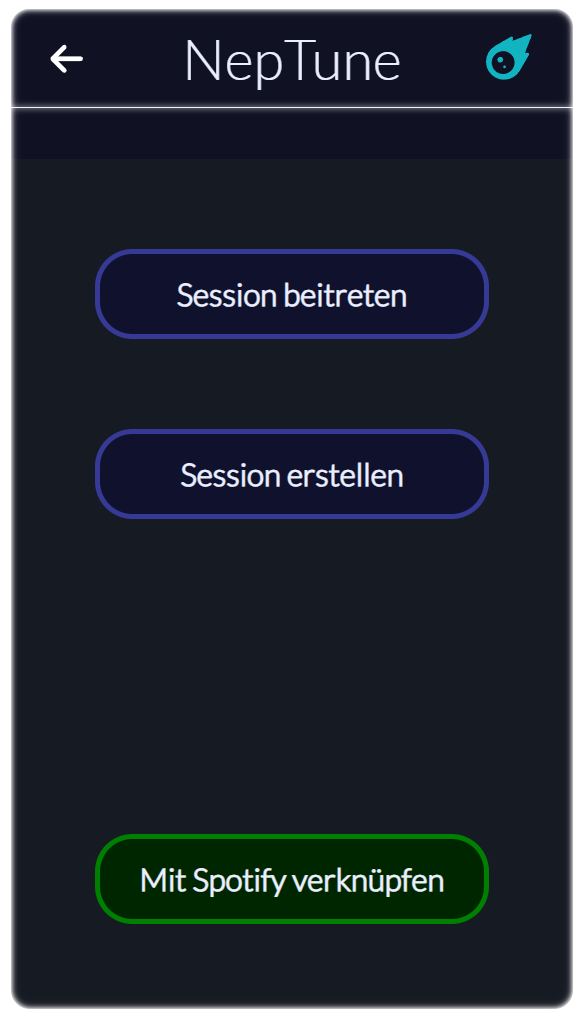
\includegraphics[width=0.4\textwidth]{LATEX/Pflichtenheft/GraphicDesigns/startPage.png}
    \captionof{figure}{startView}
\end{center}

\textbf{<Button> Session beitreten:}
\begin{itemize}
    \item Solange der User sich nicht mit einem Spotify-Account verknüpft hat, wird unter dem Button ein Hinweis angezeigt, dass User ohne verknüpften Account nur über die von anderen Usern vorgeschlagene Tracks abstimmen können. Zum Vorschlagen neuer Tacks wird ein verknüpfter Spotify-Account benötigt.
    \hypertarget{<F 1.1>}{}
    \item <F 1.1> Durch Klicken des Buttons ''Session beitreten'' gelangt der User auf die \hyperlink{joinSessionView}{joinSessionView (A 3.2)}. Dabei wird er zum Full Participant, wenn er mit einem Spotify-Account verknüpft ist. Anderfalls wird er zu einem Restricted Partcipant.
\end{itemize}

\textbf{<Button> Session erstellen:}
\begin{itemize}
    \item Der Button ''Session erstellen'' ist so lange deaktiviert und verblasst, bis sich der User über den Button ''Mit Spotify verknüpfen'' erfolgreich mit einem Spotify-Premium-Account verknüpft hat. Danach wird der Button funktionsfähig.
    \item Solange der Button ''Session erstellen'' deaktiviert ist, wird darunter ein Hinweis angezeigt, dass das Erstellen einer Session nur mit einem verknüpften Spotify-Premium-Account möglich ist.
    \hypertarget{<F 1.2>}{}
    \item <F 1.2> Durch Klicken des funktionsfähigen Buttons ''Session erstellen'' gelangt der User auf die \hyperlink{joinSessionView}{joinSessionView (A 3.5)}.
\end{itemize}

\textbf{<Button> Mit Spotify verknüpfen / Von Spotify trennen:}
\begin{itemize}
    \hypertarget{<F 1.3.A>}{}
    \item <F 1.3.A> Durch Klicken des Buttons ''Mit Spotify verknüpfen'' verknüpft sich die App, wenn möglich automatisch und im Hintergrund mit dem lokal angemeldeten Spotify-Account. Ist dies nicht möglich öffnet sich die von Spotify zur Verfügung gestellte Anmeldemaske, um per Login seinen Account zu verknüpfen.
    \item Nach dem erfolgreichen Verknüpfen mit Spotify, ändert sich die Beschriftung des Buttons von ''Mit Spotify verknüpfen'' zu ''Von Spotify trennen''.
    \hypertarget{<F 1.3.B>}{}
    \item <F 1.3.B> Durch Klicken des Buttons ''Von Spotify trennen'' wird das Spotify Konto des Users wieder von Neptune getrennt.
    \item Nach dem erfolgreichen Trennen von Spotify, ändert sich die Beschriftung des Buttons von ''Von Spotify trennen'' zu ''Mit Spotify verknüpfen''.
\end{itemize}

\textbf{<Button> Zurück:}
\begin{itemize}
\hypertarget{<F 1.4>}{}
    \item <F 1.4> Beim Klicken des Zurück-Buttons erscheint ein Pop-Up Fenster mit der Frage ''Neptune wirklich schließen?''. In diesem Pop-Up kann sich der User nun zwischen ''Ja'' und ''Nein'' entscheiden.
    \begin{itemize}
        \hypertarget{<F 1.4.A>}{}
        \item <F 1.4.A> Durch Auswählen von ''Ja'' verlässt der User die App und die App wird beendet.
        \hypertarget{<F 1.4.B>}{}
        \item <F 1.4.B> Durch Auswählen von ''Nein'' bleibt der User in der \hyperlink{startView}{startView (A 3.1)}.
    \end{itemize}
\end{itemize}



\subsection{Sessionbeitritt (joinSessionView)}
\label{sec:Benutzeroberfläche:joinSessionView}


\begin{center}
    \hypertarget{joinSessionView}{}
    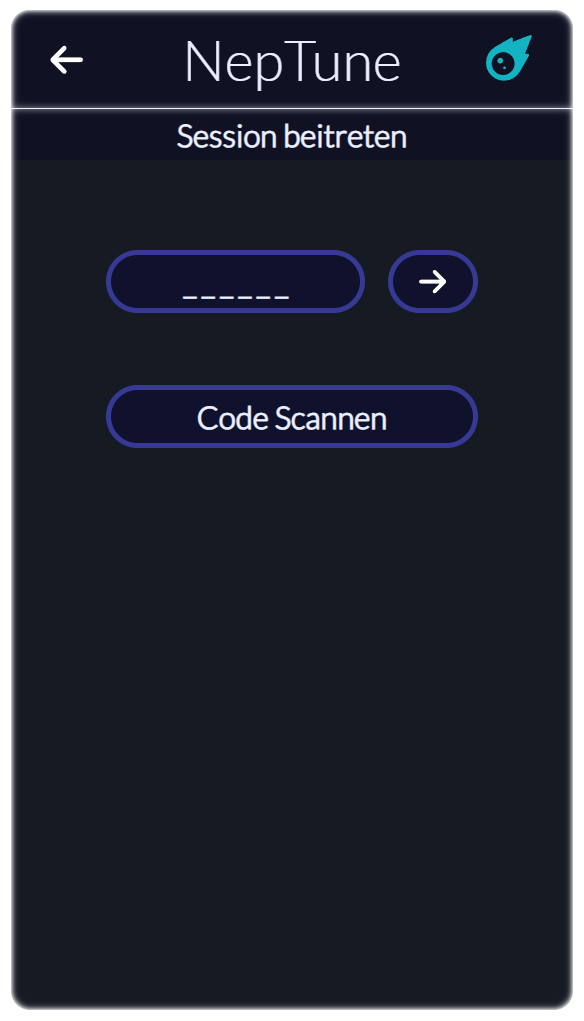
\includegraphics[width=0.4\textwidth]{LATEX/Pflichtenheft/GraphicDesigns/userJoinGroupPage.png}
    \captionof{figure}{joinSessionView}
\end{center}

\textbf{<Eingabefeld> Code-Eingabe:}
\begin{itemize}
    \item Eingabefeld zur Eingabe des sechsstelligen Codes, der die Session eindeutig identifiziert.
    \hypertarget{<F 2.1>}{}
    \item <F 2.1> Durch Anklicken des Code-Eingabefelds öffnet sich bei dem User die ''Ziffernblock-Tastatur'', mit welcher der User nun den sechsstelligen Code eingeben kann.
\end{itemize}

\textbf{<Button> Code bestätigen:}
\begin{itemize}
    \hypertarget{<F 2.2.A>}{}
    \item <F 2.2.A> Existiert eine Session zum eingegebenen sechsstelligen Code, führt Klicken des Bestätigungsbuttons auf die \hyperlink{sessionVoteView}{sessionVoteView (A 3.3)} der Session.
    \hypertarget{<F 2.2.B>}{}
    \item <F 2.2.B> Existiert keine Session zur Eingabe, erscheint ein entsprechender Hinweis unter dem Code-Eingabefeld und der Inhalt des Code-Eingabefeldes wird gelöscht.
\end{itemize}

\textbf{<Button> Code scannen:}
\begin{itemize}
    \hypertarget{<F 2.3>}{}
    \item <F 2.3> Durch Klicken des Buttons ''Code scannen'' öffnet sich ein QR-Code-Reader. Nach dem erfolgreichen Scannen eines gültigen QR-Codes gelangt man ebenfalls auf die \hyperlink{sessionVoteView}{sessionVoteView (A 3.3)} der Session.
    \hypertarget{<F 2.4>}{}
    \item <F 2.4> Der sich nach dem Klicken öffnende QR-Code-Reader besitzt einen Zurück-Button, mit dem sich der Reader wieder schließen lässt.
    \item Der sich nach dem Klicken öffnende QR-Code-Reader zeigt eine Meldung mit entsprechendem Hinweis an, falls ein erfolgreich gelesener QR-Code keinen gültigen Session-Code darstellt.
\end{itemize}

\textbf{<Button> Zurück:}
\begin{itemize}
    \hypertarget{<F 2.5>}{}
    \item <F 2.5> Durch Klicken des Zurück-Buttons gelangt man auf die \hyperlink{startView}{startView (A 3.1)}.
\end{itemize}



\subsection{Abstimmungsansicht einer Session (sessionVoteView)}
\label{sec:Benutzeroberfläche:sessionVoteView}

\begin{center}
    \hypertarget{sessionVoteView}{}
    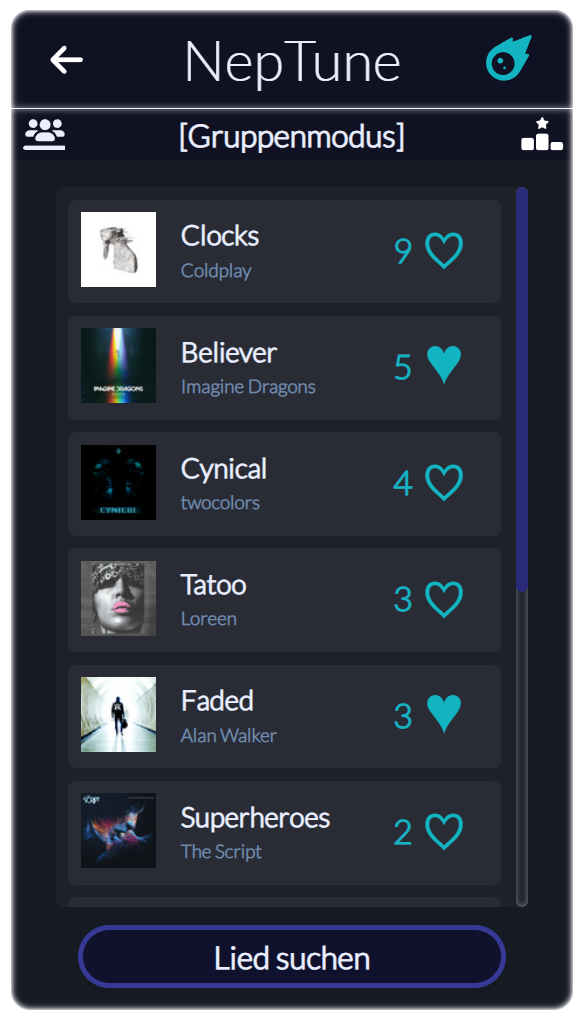
\includegraphics[width=0.4\textwidth]{LATEX/Pflichtenheft/GraphicDesigns/userVotePage.png}
    \captionof{figure}{sessionVoteView}
\end{center}

\textbf{<Button> Session-Info:}
\begin{itemize}
    \hypertarget{<F 3.1>}{}
    \item <F 3.1> Durch Klicken auf den Button Session-Info (der mit dem Gruppen-Icon) gelangt man in die \hyperlink{sessionInfoView}{sessionInfoView (A 3.9)}.
\end{itemize}

\textbf{<Textanzeige> Session-Modus:}
\begin{itemize}
    \item Zeigt den Modus der aktuellen Session an.
\end{itemize}

\textbf{<Button> Statistiken:}
\begin{itemize}
    \hypertarget{<F 3.2>}{}
    \item <F 3.2> Durch Klicken auf den Button Statistiken (der mit dem Balken-Icon) gelangt man in die \hyperlink{sessionStatsView}{sessionStatsView (A 3.10)}.
\end{itemize}

\textbf{<Track-Liste> Vorschlagsliste:}
\begin{itemize}
    \item Die Sammlung der angezeigten Tracks ist die Vorschlagsliste.
    \hypertarget{<F 3.3.A>}{} 
    \hypertarget{<F 3.3.B>}{}
    \item <F 3.3.A> bzw. <F 3.3.B> beschreiben das Klicken auf den Upvote-Button, um einen Upvote hinzuzufügen bzw. zu entfernen.
\end{itemize}

\textbf{<Button> Track suchen:}
\begin{itemize}
    \hypertarget{<F 3.4>}{}
    \item <F 3.4> Durch Klicken des Buttons ''Track suchen'' gelangt man in die \hyperlink{participantSearchView}{participantSearchView (A 3.4)}.
\end{itemize}

\textbf{<Button> Zurück:}
\begin{itemize}
    \hypertarget{<F 3.5>}{}
    \item <F 3.5> Beim Klicken des Zurück-Buttons erscheint ein Pop-Up Fenster mit der Frage ''Session wirklich verlassen?''. In diesem Pop-Up kann sich der Participant nun zwischen ''Ja'' und ''Nein'' entscheiden.
    \begin{itemize}
        \hypertarget{<F 3.5.A>}{}
        \item <F 3.5.A> Durch Auswählen von ''Ja'' verlässt die Session und gelangt in die \hyperlink{sessionStatsView}{sessionStatsView (A 3.10)}.
        \item \hypertarget{<F 3.5.B>}{} <F 3.5.B> Durch Auswählen von ''Nein'' bleibt der Participant in der \hyperlink{sessionVoteView}{sessionVoteView (A 3.3)}.
    \end{itemize}
\end{itemize}

\subsection{Tracksuche für Participants (participantSearchView)}
\label{sec:Benutzeroberfläche:participantSearchView}


\begin{center}
    \hypertarget{participantSearchView}{}
    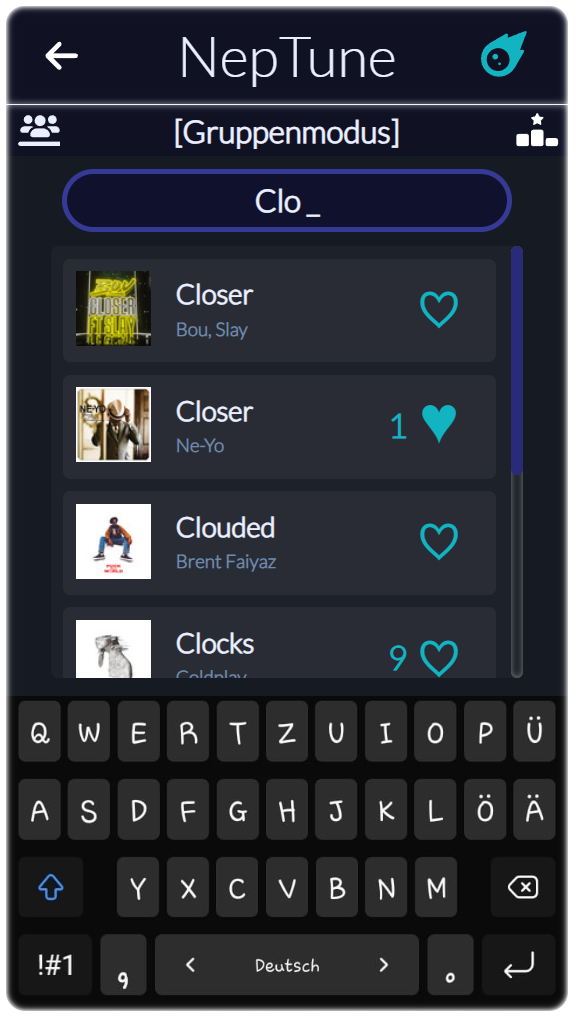
\includegraphics[width=0.4\textwidth]{LATEX/Pflichtenheft/GraphicDesigns/userSearchPage.png}
    \captionof{figure}{participantSearchView}
\end{center}

\textbf{<Button> Session-Info:}
\begin{itemize}
    \hypertarget{<F 4.1>}{}
    \item <F 4.1> Durch Klicken auf den Button Session-Info (der mit dem Gruppen-Icon) gelangt man in die \hyperlink{sessionInfoView}{sessionInfoView (A 3.9)}.
\end{itemize}

\textbf{<Textanzeige> Session-Modus:}
\begin{itemize}
    \item Zeigt den Modus der aktuellen Session an.
\end{itemize}

\textbf{<Button> Statistiken:}
\begin{itemize}
    \hypertarget{<F 4.2>}{}
    \item <F 4.2> Durch Klicken auf den Button Statistiken (der mit dem Balken-Icon) gelangt man in die \hyperlink{sessionStatsView}{sessionStatsView (A 3.10)}.
\end{itemize}

\textbf{<Eingabefeld> Track-Suchbegriff:}
\begin{itemize}
    \item Eingabefeld für den Eingabebegriff zur Suche nach Tracks.
    \hypertarget{<F 4.3>}{}
    \item <F 4.3> Ändert sich der Eingabebegriff, werden die Track-Suchergebnisse aktualisiert.
    \item Die Tastatur wird standardmäßig beim Wechsel in die \hyperlink{participantSearchView}{participantSearchView (A 3.4)} geöffnet.
\end{itemize}

\textbf{<Track-Liste> Track-Suchergebnisse:}
\begin{itemize}
    \item Die Sammlung der angezeigten Tracks ist bei Full Participants der gesamte Musikkatalog von Spotify, mit den zum Suchbegriff passenden Tracks. Dabei gelten folgende Einschränkungen:
    \begin{itemize}
        \item Im General Mode gibt es keine Einschränkungen.
        \item Im Artist Mode werden nur Tracks der vom Host bei \hyperlink{hostModeSettingsView}{Sessionerstellung (A 3.6)} definierten Artists angezeigt.
        \item Im Genre Mode werden nur Tracks der vom Host bei \hyperlink{hostModeSettingsView}{Sessionerstellung (A 3.6)} definierten Genres angezeigt.
        \item Im Playlist Mode werden nur Tracks der vom Host bei \hyperlink{hostModeSettingsView}{Sessionerstellung (A 3.6)} definierten Playlist angezeigt.
    \end{itemize}
    \item Die Sammlung der angezeigten Tracks ist bei Restricted Participants nur die Vorschlagsliste.
    \hypertarget{<F 4.4.A>}{}
    \hypertarget{<F 4.4.B>}{}
    \item <F 4.4.A> bzw. <F 4.4.B> beschreiben das Klicken auf den Upvote-Button, um einen Upvote hinzuzufügen bzw. zu entfernen.
\end{itemize}

\textbf{<Button> Zurück:}
\begin{itemize}
    \hypertarget{<F 4.5>}{}
    \item <F 4.5> Durch Klicken des Zurück-Buttons gelangt man in die  \hyperlink{sessionVoteView}{sessionVoteView (A 3.3)}.
\end{itemize}


\subsection{Moduswahl für den Host (hostModeSelectView)}
\label{sec:Benutzeroberfläche:hostModeSelectView}


\begin{center}
    \hypertarget{hostModeSelectView}{}
    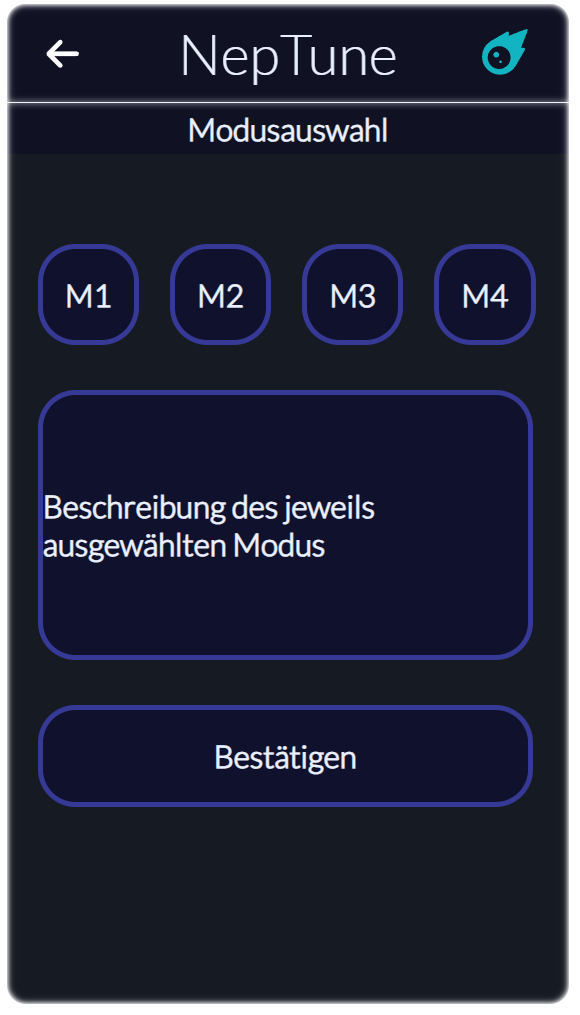
\includegraphics[width=0.4\textwidth]{LATEX/Pflichtenheft/GraphicDesigns/hostModusSelectPage.png}
    \captionof{figure}{hostModeSelectView}
\end{center}

\textbf{<Buttons> Modus-Buttons:}
\begin{itemize}
    \item Es stehen vier Modus-Buttons zur Verfügung:
    \begin{itemize}
        \item Der erste Button ist für den General Mode \hyperlink{General Mode}{(Use-Case-Diagramm (A 4.2))}
        \item Der zweite Button ist für den Artist Mode \hyperlink{Artist Mode}{(Use-Case-Diagramm (A 4.3))}
        \item Der dritte Button ist für den Genre Mode \hyperlink{Genre Mode}{(Use-Case-Diagramm (A 4.4))}
        \item Der vierte Button ist für den Playlist Mode \hyperlink{Playlist Mode}{(Use-Case-Diagramm (A 4.5))}
    \end{itemize}
    \item \hypertarget{<F 5.1.M>}{} <F 5.1.A/B/C/D> Durch Klicken auf einen der vier Modus-Buttons wird dieser markiert. Es kann stets nur ein Modus-Button markiert sein. Zu Beginn ist der erste Button markiert. Der Modus des markierten Buttons ist angewählt.
\end{itemize}

\textbf{<Textanzeige> Modus-Info-Anzeige:}
\begin{itemize}
    \item Die Anzeige beinhaltet eine kurze Beschreibung des angewählten Modus.
\end{itemize}

\textbf{<Button> Bestätigen:}
\begin{itemize}
    \item <F 5.2> Durch Klicken des Bestätigen-Buttons wird der angewählte Modus übernommen und der Host gelangt in die \hyperlink{hostModeSettingsView}{hostModeSettingsView (A 3.6)}.
\end{itemize}

\textbf{<Button> Zurück:}
\begin{itemize}
    \item <F 5.3> Durch Klicken des Zurück-Buttons gelangt man in die  \hyperlink{startView}{startView (A 3.1)}.
\end{itemize}



\subsection{Moduseinstellungen für den Host (hostModeSettingsView)}
\label{sec:Benutzeroberfläche:hostModeSettingsView}

\begin{center}
    \hypertarget{hostModeSettingsView}{}
    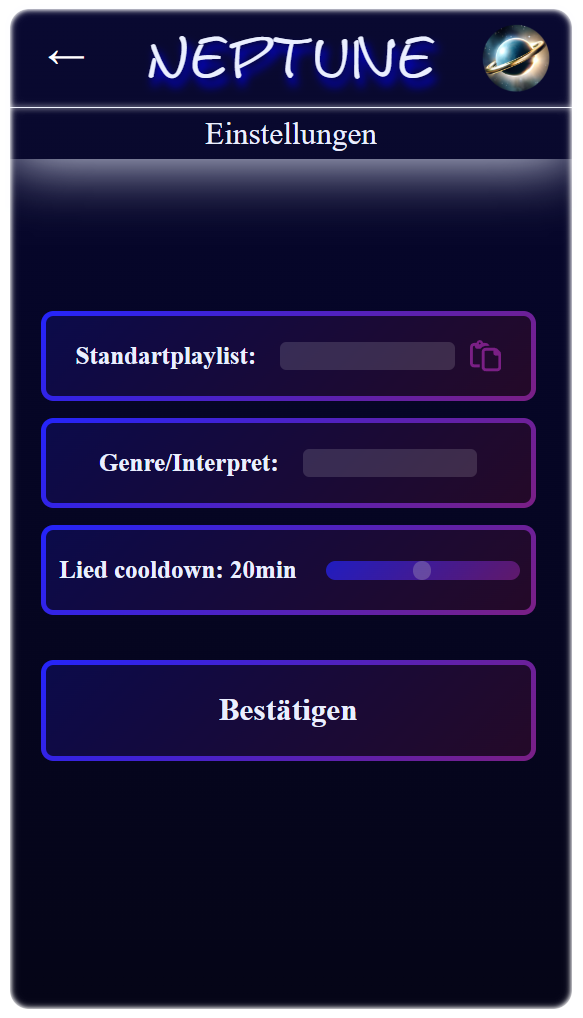
\includegraphics[width=0.4\textwidth]{LATEX/Pflichtenheft/GraphicDesigns/hostModusSettingsPage.png}
    \captionof{figure}{hostModeSettingsView}
\end{center}

\textbf{<Eingabefeld> Playlist-Link:}
\begin{itemize}
    \item <F 6.1> Eingabefeld zum Einfügen eines gültigen Spotify-Share-Links der gewünschten Playlist.
    \item Dieses Feld muss im Playlistmodus gefüllt werden, darf aber auch in jedem anderen Modus benutzt werden. Wurde eine Playlist in einem anderem Modus als dem Playlist-Mode eingegeben, dient diese als Quelle für weitere Tracks der Queue, falls die Queue leer ist und sich keine Tracks mehr in der Vorschlagsliste befinden.
\end{itemize}

\textbf{<Button> Artist-Auswahl:}
\begin{itemize}
    \item Nur im Artist Mode vorhanden.
    \item <F 6.2.A> Durch Klicken der Artist-Auswahl gelangt man in die \hyperlink{artistSelectView}{artistSelectView (3.2.11)}.
\end{itemize}

\textbf{<Abwandlung der Track-Liste> Artist-Liste:}
\begin{itemize}
    \item Nur im Artist Mode vorhanden.
    \item Statt Tracks werden Artists mit Bild und Name angezeigt. Statt dem Herz wird ein Plus-Symbol angezeigt. Ansonsten bleibt das Layout gleich. Ein Menü-Button für Artists existiert nicht.
    \item Die Sammlung der angezeigten Artists sind die in der \hyperlink{artistSelectView}{artistSelectView (3.2.11)} bereits ausgewählten Artists. 
    \item <F 6.3.A> das Klicken auf den Plus-Button, um einen Artist zu entfernen.
\end{itemize}

\textbf{<Button> Genre-Auswahl:}
\begin{itemize}
    \item Nur im Genre Mode vorhanden.
    \item <F 6.2.B> Durch Klicken der Genre-Auswahl gelangt man in die  \hyperlink{genreSelectView}{genreSelectView (3.2.12)}.
\end{itemize}

\textbf{<Abwandlung der Track-Liste> Genre-Liste:}
\begin{itemize}
    \item Nur im Genre Mode vorhanden.
    \item Statt Tracks werden Genres angezeigt. Ansonsten bleibt das Layout gleich. Ein Menü-Button für Genres existiert nicht.
    \item Die Sammlung der angezeigten Genres sind die in der \hyperlink{genreSelectView}{genreSelectView (3.2.12)} bereits ausgewählten Genres. 
    \item <F 6.3.B> das Klicken auf den Plus-Button, um ein Genre zu entfernen.
\end{itemize}

\textbf{<Slider> Track-Cooldown:}
\begin{itemize}
    \item In jedem Modus vorhanden.
    \item <F 6.4> Ein Slider zur Auswahl des zeitlichen Cooldowns bis ein gespielter Track erneut zum Upvoten verfügbar wird.
    \item Der derzeit eingestellte Wert wird neben dem Slider angezeigt.
    \item Der Wertebereich des Sliders geht von 0 Minuten bis 12 Stunden und verläuft nicht linear, sondern eher aber möglicherweise nicht exakt exponentiell.
\end{itemize}

\textbf{<Button> Bestätigen:}
\begin{itemize}
    \item Der Bestätigen-Button ist zunächst verblasst und nicht klickbar. Er wird erst klickbar, nachdem je nach Modus eine Playlist, mindestens ein Artist oder mindestens ein Genre eingestellt wurden.
    \item <F 6.5> Durch Klicken des Bestätigen-Buttons werden die Einstellungen angewendet und die Session eröffnet. Der Host gelangt in die \hyperlink{hostControlView}{hostControlView (A 3.7)}.
\end{itemize}

\textbf{<Button> Zurück:}
\begin{itemize}
    \item <F 6.6> Durch Klicken des Zurück-Buttons gelangt man in die  \hyperlink{joinSessionView}{joinSessionView (A 3.5)}.
\end{itemize}



\subsection{Kontrollansicht für den Host (hostControlView)}
\label{sec:Benutzeroberfläche:hostControlView}

\begin{center}
    \hypertarget{hostControlView}{}
    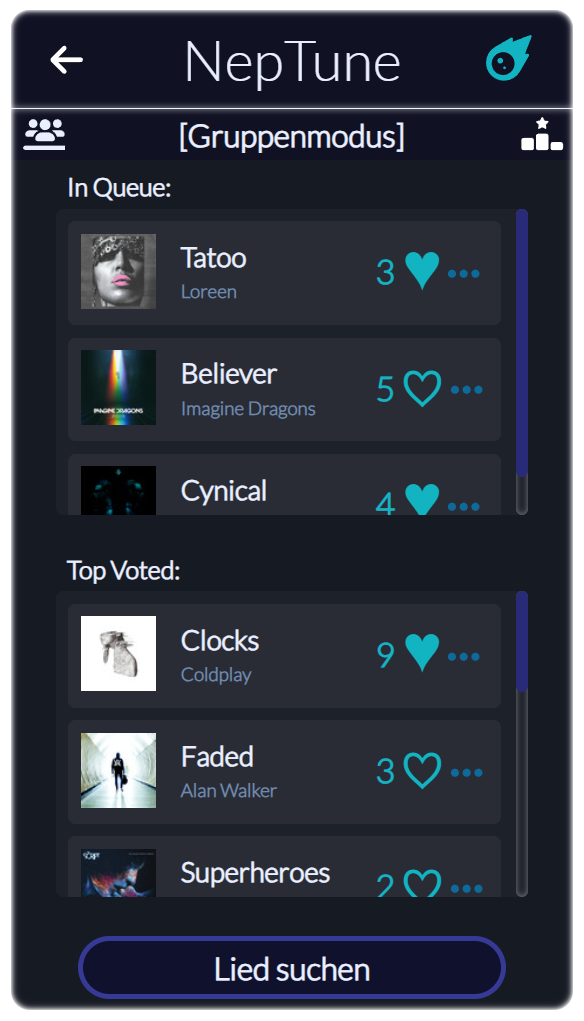
\includegraphics[width=0.4\textwidth]{LATEX/Pflichtenheft/GraphicDesigns/hostControlPage.png}
    \captionof{figure}{hostControlView}
\end{center}

\textbf{<Button> Session-Info:}
\begin{itemize}
    \item <F 7.1> Durch Klicken auf den Button Session-Info (der mit dem Gruppen-Icon) gelangt man in die \hyperlink{sessionInfoView}{sessionInfoView (A 3.9)}.
\end{itemize}

\textbf{<Textanzeige> Session-Modus:}
\begin{itemize}
    \item Zeigt den Modus der aktuellen Session an.
\end{itemize}

\textbf{<Button> Statistiken:}
\begin{itemize}
    \item <F 7.2> Durch Klicken auf den Button Statistiken (der mit dem Balken-Icon) gelangt man in die \hyperlink{sessionStatsView}{sessionStatsView (A 3.10)}.
\end{itemize}

\textbf{<Track-Liste> Queue-Anzeige:}
\begin{itemize}
    \item Die Sammlung der angezeigten Tracks ist die Queue.
    \item <F 7.3.A> bzw. <F 7.3.B> beschreiben das Klicken auf den Upvote-Button, um einen Upvote hinzuzufügen bzw. zu entfernen.
    \item <F 7.4> Der Track-Menü-Button bietet folgende Auswahlmöglichkeiten:
    \begin{itemize}
        \hypertarget{<F 7.4.A>}{}
        \item <F 7.4.A> Track aus Queue entfernen
        \hypertarget{<F 7.4.B>}{}
        \item <F 7.4.B> Track sperren
    \end{itemize}
    \hypertarget{<F 7.5>}{}
    \item <F 7.5> Jeder Track lässt sich per Drag-and-Drop innerhalb der Queue-Anzeige verschieben, um die Reihenfolge anzupassen.
\end{itemize}

\textbf{<Track-Liste> Vorschlagsliste:}
\begin{itemize}
    \item Die Sammlung der angezeigten Tracks ist die Vorschlagsliste.
    \hypertarget{<F 7.6.A>}{}
    \hypertarget{<F 7.6.B>}{}
    \item <F 7.6.A> bzw. <F 7.6.B> beschreiben das Klicken auf den Upvote-Button, um einen Upvote hinzuzufügen bzw. zu entfernen.
    \hypertarget{<F 7.7>}{}
    \item <F 7.7> Der Track-Menü-Button bietet folgende Auswahlmöglichkeiten:
    \begin{itemize}
        \hypertarget{<F 7.7.A>}{}
        \item <F 7.7.A> Track unten zur Queue hinzufügen (Nur verfügbar, falls sich der Track noch nicht in der Queue befindet)
        \hypertarget{<F 7.7.B>}{}
        \item <F 7.7.B> Track sperren
    \end{itemize}
    \hypertarget{<F 7.8>}{}
    \item <F 7.8> Jeder Track lässt sich per Drag-and-Drop an eine bestimmte Stelle der Queue-Anzeige verschieben, um ihn an dieser Stelle in der Queue zu positionieren.
\end{itemize}

\textbf{<Button> Track suchen:}
\begin{itemize}
    \hypertarget{<F 7.9>}{}
    \item <F 7.9> Durch Klicken des Buttons ''Track suchen'' gelangt man in die \hyperlink{hostSearchView}{hostSearchView (A 3.8)}.
\end{itemize}

\textbf{Zurück-Button:}
\begin{itemize}
    \hypertarget{<F 7.10>}{}
    \item <F 7.10> Beim Klicken des Zurück-Buttons erscheint ein Pop-Up Fenster mit der Frage ''Session wirklich löschen?''. In diesem Pop-Up kann sich der Host nun zwischen ''Ja'' und ''Nein'' entscheiden.
    \begin{itemize}
    \hypertarget{<F 7.10.A>}{}
        \item <F 7.10.A> Durch Auswählen von ''Ja'' wird die Session gelöscht und der Host gelangt in die \hyperlink{sessionStatsView}{sessionStatsView (A 3.10)}. Auch alle Participants der Session gelangen in die \hyperlink{sessionStatsView}{sessionStatsView (A 3.10)}.
        \hypertarget{<F 7.10.B>}{}
        \item <F 7.10.B> Durch Auswählen von ''Nein'' bleibt der Host in der \hyperlink{hostControlView}{hostControlView (A 3.7)}.
    \end{itemize}
\end{itemize}

\subsection{Tracksuche für den Host (hostSearchView)}
\label{sec:Benutzeroberfläche:hostSearchView}


\begin{center}
    \hypertarget{hostSearchView}{}
    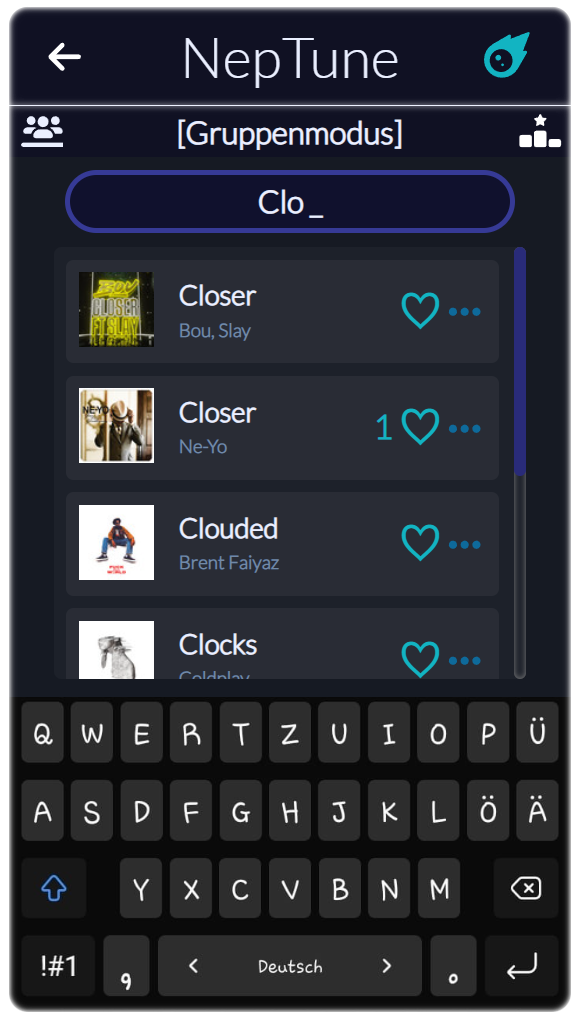
\includegraphics[width=0.4\textwidth]{LATEX/Pflichtenheft/GraphicDesigns/hostSearchPage.png}
    \captionof{figure}{hostSearchView}
\end{center}

Die hostSearchView ist identisch zur \hyperlink{participantSearchView}{participantSearchView (A 3.4)}, die Testfälle seien hier mit <F 8.1> bis <F 8.3> als F-Nummern versehen. Ausnahmen sind folgende Elementen, die anders definiert sind bzw. zusätzlich vorhanden sind:

\textbf{<Track-Liste> Track-Suchergebnisse:}
\begin{itemize}
    \item Die Sammlung der angezeigten Tracks ist gesamte Musikkatalog von Spotify, mit den zum Suchbegriff passenden Tracks. Dabei gelten ebenjene Einschränkungen aus der \hyperlink{participantSearchView}{participantSearchView (A 3.4)}.
    \hypertarget{<F 8.4.A>}{}
    \hypertarget{<F 8.4.B>}{}
    \item <F 8.4.A> bzw. <F 8.4.B> beschreiben das Klicken auf den Upvote-Button, um einen Upvote hinzuzufügen bzw. zu entfernen.
    \hypertarget{<F 8.5>}{}
    \item <F 8.5> Der Track-Menü-Button bietet folgende Auswahlmöglichkeiten:
    \begin{itemize}
    \hypertarget{<F 8.5.A>}{}
        \item <F 8.5.A> Track hinten in die Queue hinzufügen (Nur möglich, falls der Track noch nicht in der Queue ist)
        \hypertarget{<F 8.5.B>}{}
        \item <F 8.5.B> Track sperren bzw. entsperren (Je nachdem ob der Track gesperrt bzw. entsperrt ist)
        \hypertarget{<F 8.5.C>}{}
        \item <F 8.5.C> Cooldown aufheben (Nur möglich, falls der Track einen Cooldown besitzt)
    \end{itemize}
\end{itemize}

\textbf{<Button> Zurück:}
\begin{itemize}
    \hypertarget{<F 8.6>}{}
    \item <F 8.6> Durch Klicken des Zurück-Buttons gelangt man in die  \hyperlink{hostControlView}{hostControlView (A 3.7)}.
\end{itemize}

\textbf{<Button> Track-Filter:}
\begin{itemize}
    \hypertarget{<F 8.7>}{}
    \item <F 8.7> Bei Anklicken des Track-Filter-Buttons (der mit dem Filter-Icon) öffnet sich ein kleines Dropdown-Menü mit zwei Auswahlmöglichkeiten zur Filter-Aktivierung:
    \begin{itemize}
        \hypertarget{<F 8.7.A>}{}
        \item <F 8.7.A> Dem Cooldown-Filter für Tracks mit Cooldown (Filter-Icon mit kleiner Uhr)
        \hypertarget{<F 8.7.B>}{}
        \item <F 8.7.B> Dem Sperr-Filter für gesperrte Tracks (Filter-Icon mit kleinem Schloss)
    \end{itemize}
    \item Durch Aktivieren werden in der Track-Anzeige nur Tracks angezeigt, welche auf den Filter zutreffen.
    \item Das angezeigte Filter-Icon ist das des aktiven Filters.
    \hypertarget{<F 8.8>}{}
    \item <F 8.8> Wird das bereits aktive Filter-Icon erneut angeklickt, so wird der Filter deaktiviert.
    \item Es kann stets nur ein Filter aktiv sein.
\end{itemize}


\subsection{Session-Info (sessionInfoView)}
\label{sec:Benutzeroberfläche:sessionInfoView}

\begin{center}
    \hypertarget{sessionInfoView}{}
    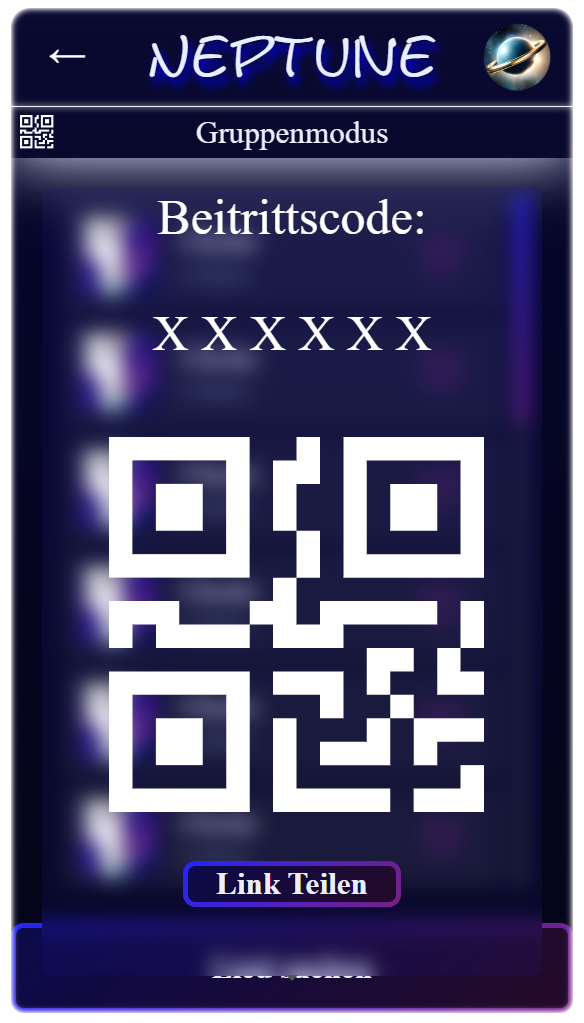
\includegraphics[width=0.4\textwidth]{LATEX/Pflichtenheft/GraphicDesigns/shareLinkPopUpPage.png}
    \captionof{figure}{sessionInfoView}
\end{center}

\textbf{<Anzeige> Sessionmodus:}
\begin{itemize}
    \item Anzeige des aktuellen Modus der Session.
\end{itemize}

\textbf{<Anzeige> Artist/Genre-Info:}
\begin{itemize}
    \item Nur im Artist oder Genre Mode: Anzeige der erlaubten Artists oder Genres.
\end{itemize}

\textbf{<Anzeige> Beitrittscode:}
\begin{itemize}
    \item Anzeige des sechsstelligen Codes zum Beitritt der Session.
\end{itemize}

\textbf{<QR-Code-Anzeige> QR-Code:}
\begin{itemize}
    \item Scannbare Anzeige des sechsstelligen Codes zum Beitritt der Session als QR-Code.
\end{itemize}

\textbf{<Anzeige> Share-Link:}
\begin{itemize}
    \item Kopierbare Anzeige eines Links zum Beitreten der Session.
\end{itemize}

\textbf{<Button> Link teilen:}
\begin{itemize}
    \item <F 9.1> Teilt beim Klicken den Link zum Beitreten der Session über die Android-Schnittstelle zum Teilen von Inhalten.
\end{itemize}

\textbf{<Button> Zurück:}
\begin{itemize}
    \hypertarget{<F 9.2>}{}
    \item <F 9.2> Durch Klicken des Zurück-Buttons gelangt man in die letzte View auf dem Backstack, von der aus die sessionInfoView geöffnet wurde.
    \item (Es wird keinen X-Button geben, obwohl dieser im Grafikentwurf gezeigt wird.)
\end{itemize}


\subsection{Session-Statistiken (sessionStatsView)}
\label{sec:Benutzeroberfläche:sessionStatsView}


\begin{center}
    \hypertarget{sessionStatsView}{}
    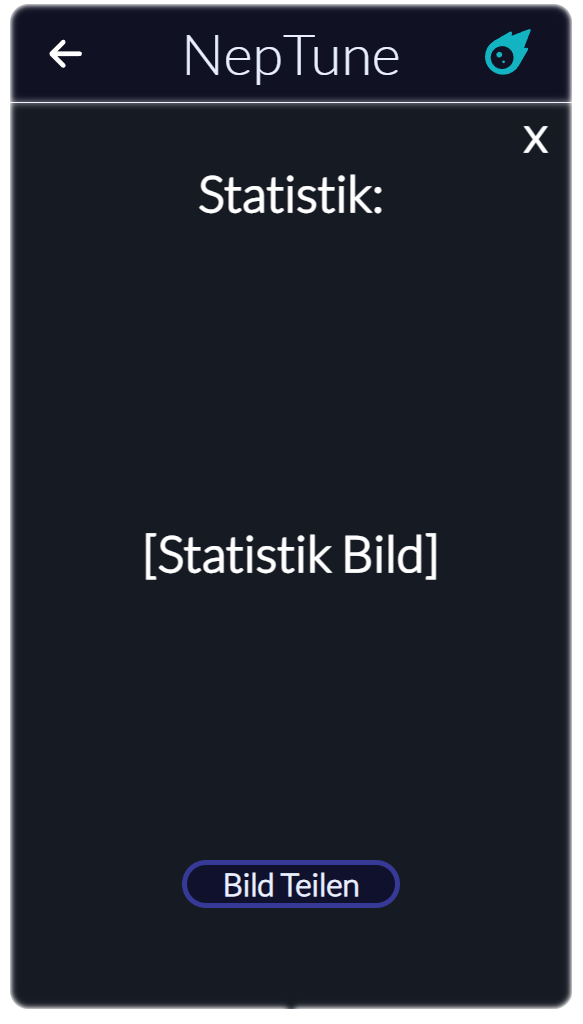
\includegraphics[width=0.4\textwidth]{LATEX/Pflichtenheft/GraphicDesigns/statisticsPopUpPage.png}
    \captionof{figure}{sessionStatsView}
\end{center}

\textbf{<Bild-Anzeige> Statistik-Bild:}
\begin{itemize}
    \item Anzeige eines generierten Bildes, das alle gewählten Statistiken über die Session aus den \hyperlink{Wunschkriterien}{Wunschkriterien (2.2)} enthält.
\end{itemize}

\textbf{<Button> Statistik-Bild teilen:}
\begin{itemize}
    \hypertarget{<F 10.1>}{}
    \item <F 10.1> Teilt beim Klicken das angezeigte Bild der Statistik über die Android-Schnittstelle zum Teilen von Inhalten.
\end{itemize}

\textbf{<Button> Zurück:}
\begin{itemize}
    \hypertarget{<F 10.2>}{}
    \item <F 10.2> Durch Klicken des Zurück-Buttons gelangt man in die letzte View auf dem Backstack, von der aus die sessionInfoView geöffnet wurde. Falls die Session nicht mehr existiert, gelangt man in die \hyperlink{startView}{startView (A 3.1)}.
    \item (Es wird keinen X-Button geben, obwohl dieser im Grafikentwurf gezeigt wird.)
\end{itemize}



\subsection{Artist-Auswahl (artistSelectView)}
\label{sec:Benutzeroberfläche:artistSelectView}
\hypertarget{artistSelectView}{}

Das Gesamtdesign dieser View ist analog zur \hyperlink{participantSearchView}{participantSearchView (A 3.4)}.

\textbf{<Eingabefeld> Artist-Suchbegriff:}
\begin{itemize}
    \item Eingabefeld für den Eingabebegriff zur Suche nach Artists.
    \item <F 11.1> Ändert sich der Eingabebegriff, werden die Track-Suchergebnisse aktualisiert.
    \item Die Tastatur wird standardmäßig beim Wechsel in die \hyperlink{artistSelectView}{artistSelectView (3.2.11)} geöffnet.
\end{itemize}

\textbf{<Abwandlung der Track-Liste> Artist-Suchergebnisse:}
\begin{itemize}
    \item Statt Tracks werden Artists mit Bild und Name angezeigt. Statt dem Herz wird ein Plus-Symbol angezeigt. Ansonsten bleibt das Layout gleich. Ein Menü-Button für Artists existiert nicht.
    \item Die Sammlung der angezeigten Artists ist der gesamte Artist-Katalog von Spotify.
    \hypertarget{<F 11.2.A>}{}
    \hypertarget{<F 11.2.B>}{}
    \item <F 11.2.A> bzw. <F 11.2.B> beschreiben das Klicken auf den Plus-Button, um einen Artist zur Auswahl hinzuzufügen bzw. zu entfernen.
\end{itemize}

\textbf{<Button> Zurück:}
\begin{itemize}
    \hypertarget{<F 11.3>}{}
    \item <F 11.3> Durch Klicken des Zurück-Buttons gelangt man in die  \hyperlink{hostModeSettingsView}{hostModeSettingsView (A 3.6)}.
\end{itemize}


\subsection{Genre-Auswahl (genreSelectView)}
\label{sec:Benutzeroberfläche:genreSelectView}
\hypertarget{genreSelectView}{}

Diese View ist identisch zur \hyperlink{artistSelectView}{artistSelectView (3.2.11)}, mit der Abwandlung, dass statt Artists Genres angezeigt werden. Die Funktionalitäten sind analog mit <F 12.1> bis <F 12.3> beschrieben.






\section{Weitere funktionale Anforderungen}
\label{sec:Benutzeroberfläche:Grafiken}

\begin{itemize}
    \hypertarget{<F 100>}
    \item <F 100> Das vollständige Beenden der App wird durch das Verlassen der \hyperlink{startView}{startView (A 3.1)} per Zurück-Button oder durch Android-System-Funktionalitäten ermöglicht.
    \item <F 101> Wenn die App vollständig beendet ist/war, öffnet sich beim Starten der App eine von drei Views:
    \hypertarget{<F 101>}{}
    \begin{itemize}
        \item Die \hyperlink{sessionVoteView}{sessionVoteView (A 3.3)} öffnet sich, wenn man derzeit Participant einer aktiven Session ist.
        \item Die \hyperlink{hostControlView}{hostControlView (A 3.7)} öffnet sich, wenn man derzeit Host einer aktiven Session ist.
        \item Die \hyperlink{startView}{startView (A 3.1)} öffnet sich, wenn man derzeit nicht Participant oder Host einer aktiven Session ist.
    \end{itemize}
    \hypertarget{<F 102>}{}
    \item <F 102> Falls die App nicht vollständig beendet wurde und die Zustandsdaten des Android-Betriebssystems noch vorhanden sind, so öffnet sich die App in der Ansicht, in der man sie verlassen hat.
    \item Beim Beginn des tatsächlichen Abspielens wird der Track aus der Queue und der Vorschlagsliste entfernt. Die vorhandenen Upvotes werden auf 0 zurückgesetzt und der Track wird mit dem vom Host bei der \hyperlink{hostModeSettingsView}{Sessionerstellung (A 3.6)} definierten Cooldown belegt.
    \item Verlässt ein Participant eine Session, werden seine Upvotes weiterhin gespeichert. Sollte der Participant dieser Session dann wieder beitreten, behält er dadurch alle seine Upvotes.
    \item Eine Session kann entweder manuell durch den Host beendet werden, indem dieser sie verlässt oder sie endet automatisch, sobald die Queue leer ist und der derzeit abgespielte Song beendet ist, während der Host die App geschlossen hat.
    \item Sobald die Queue leer ist und der Host erreichbar ist (d.h. die App ausgeführt wird), wird der meist upgevotetste Track automatisch der Queue hinzugefügt. Hat kein Track mehr ein Upvote, wird ein Track aus der hinterlegten Playlist der Queue hinzugefügt. Wurde keine Playlist hinterlegt, so wird ein Track aus der Spotify Autoplay Funktion hinzugefügt. Sollte sich ein neuer meistgeupvoteter Track ergeben, wird die Queue aktualisiert, falls der Host erreichbar ist.
    \item Sobald die Session beendet wird, gelangen alle Particpants und der Host der Session in die \hyperlink{sessionStatsView}{sessionStatsView (A 3.10)}.
    \item Die Anzeigesprache der App ist Deutsch, wenn Deutsch als Systemsprache des Geräts eingestellt ist. Falls eine andere Sprache als Systemsprache eingestellt ist, ist die Anzeigesprache der App Englisch.
    \item Die Verknüfung mit oder Trennung von Spotify wird dauerhaft gespeichert, auch nach vollständigem Beenden der App.
\end{itemize}






% show subsections in contents
\addtocontents{toc}{\protect\setcounter{tocdepth}{2}}
\chapter{Anwendungsfälle}
\hypertarget{Anwendungsfaelle}{}
\label{chap:Anwendungsfälle}

In diesem Kapitel werden einige Anwendungsfälle der App mithilfe von Use Case Diagrammen anschaulich gemacht. Diese beschreiben das Starten einer Session, sowie die einzelnen Modi der App.

\section{Session erstellen}
\label{sec:Anwendungsfälle:Session erstellen}
\hypertarget{Session erstellen}{}

\begin{figure}[h]
    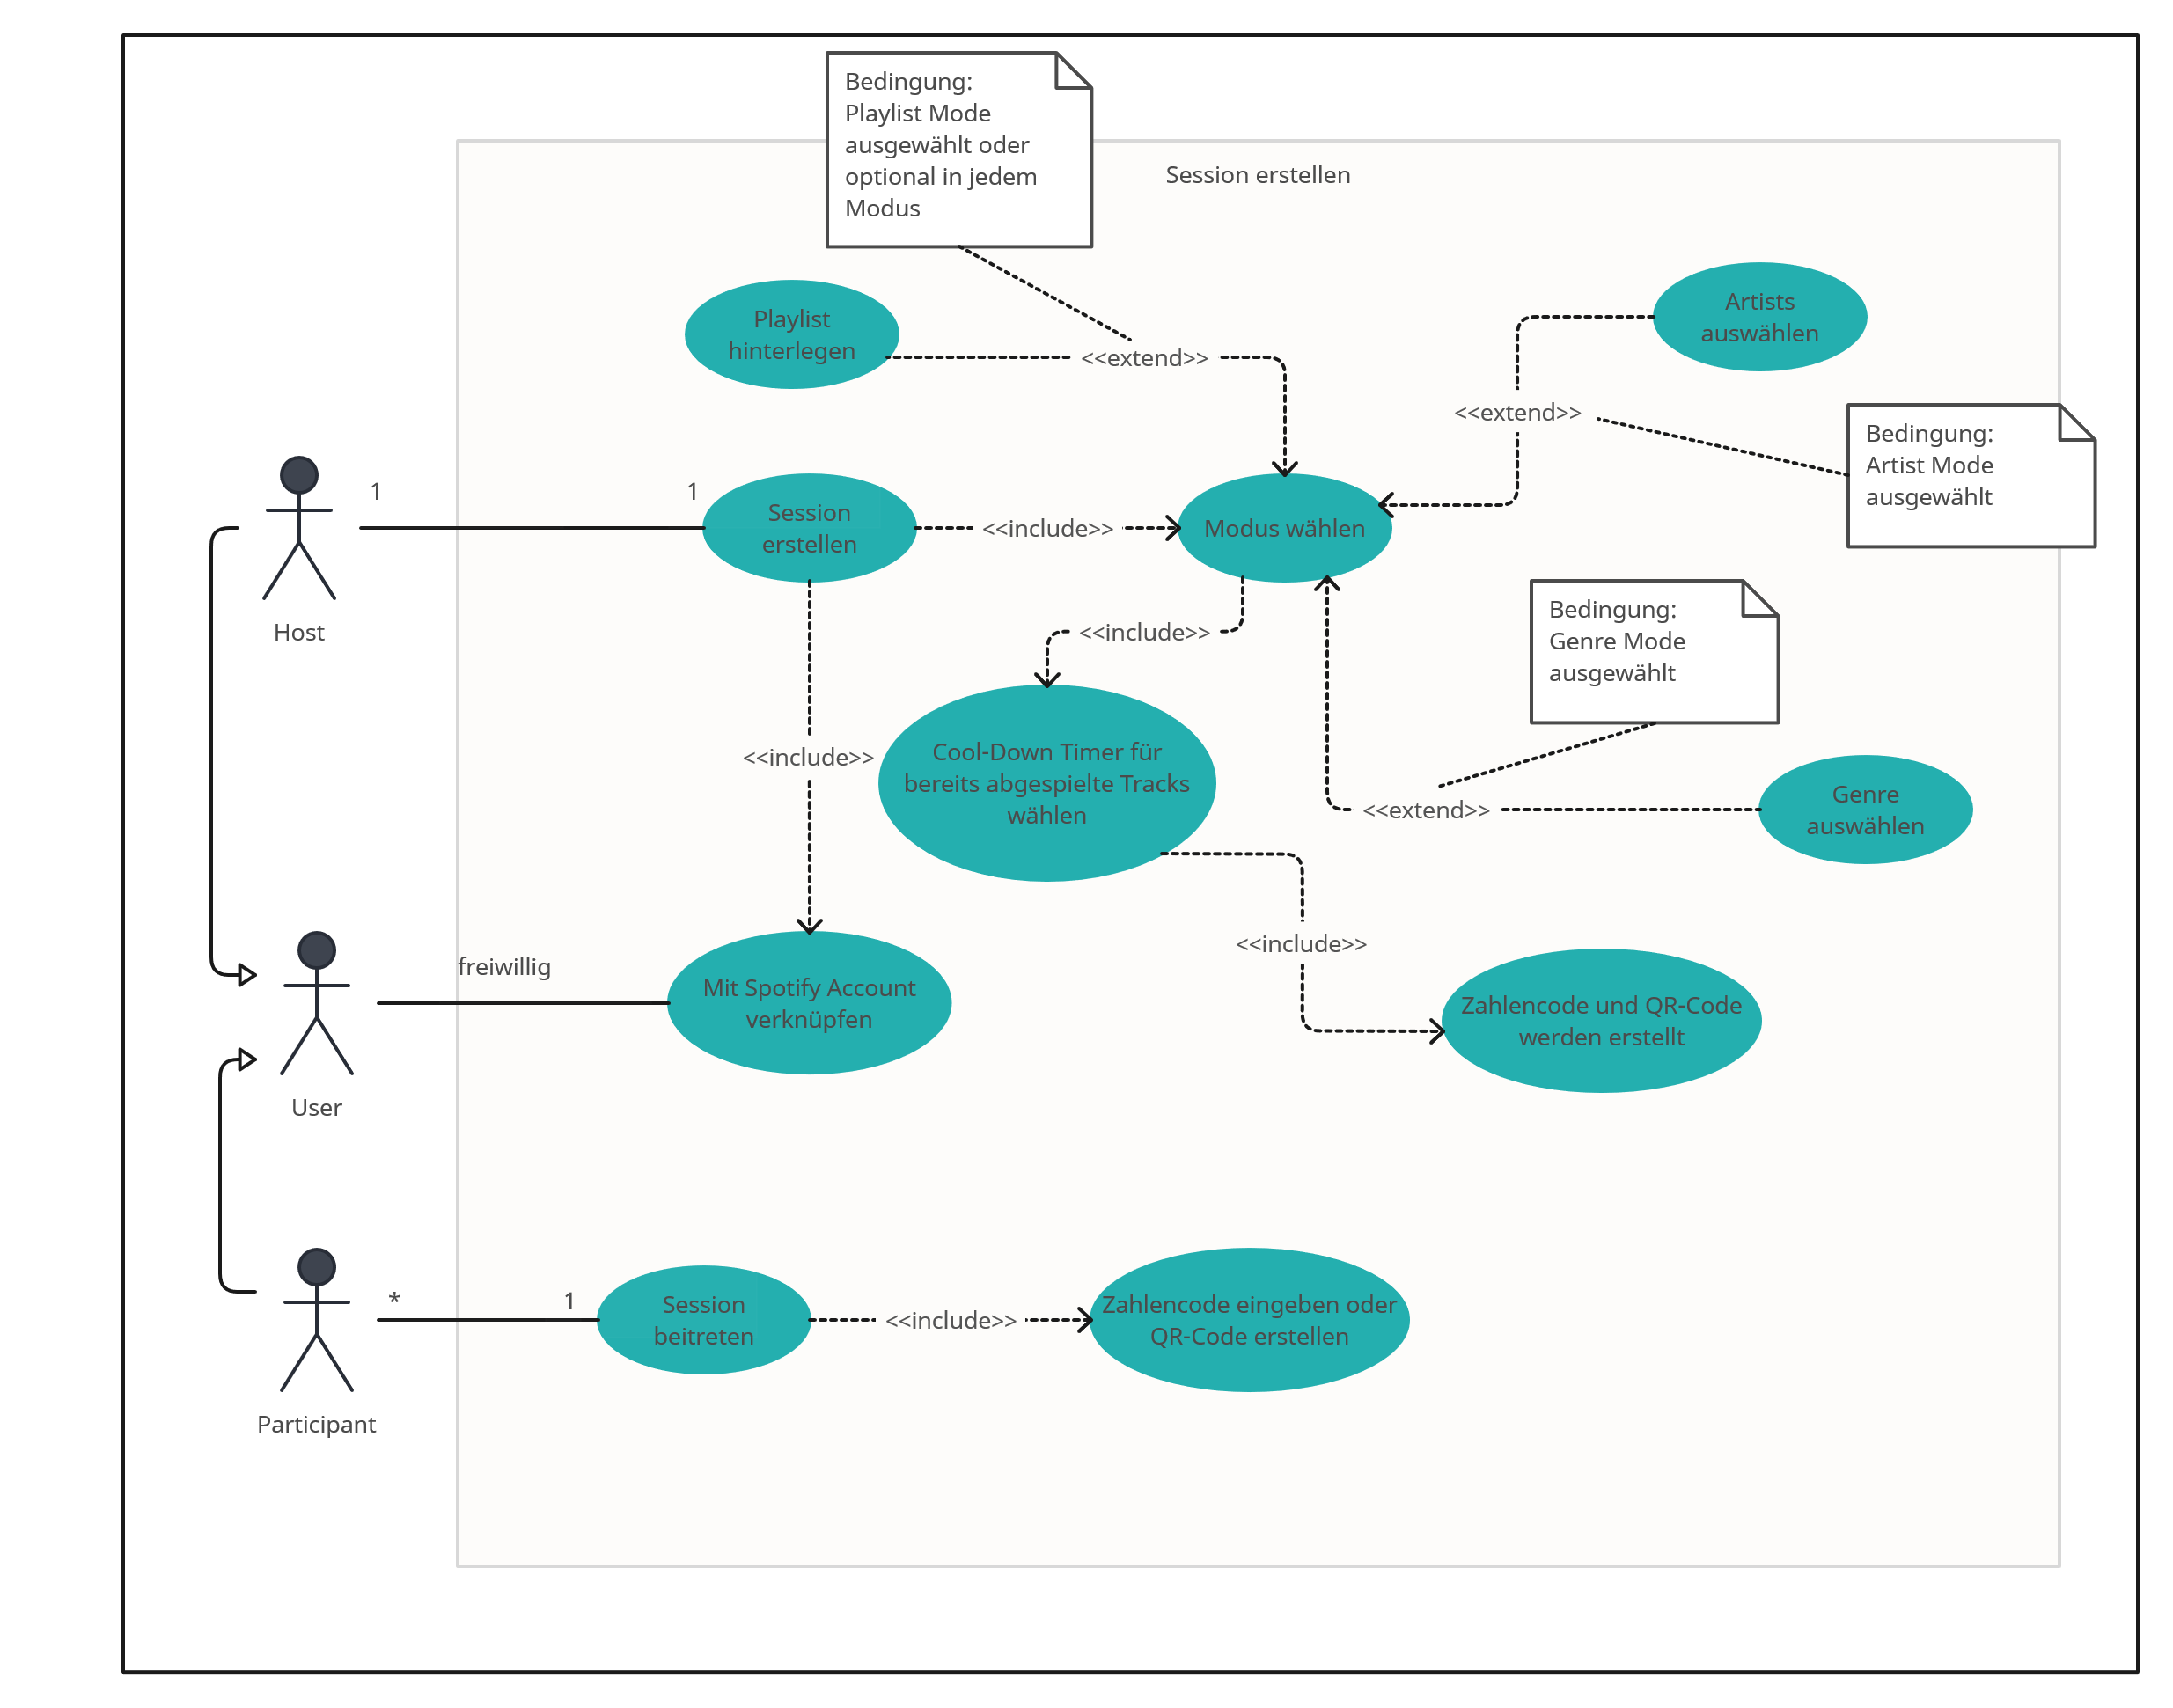
\includegraphics[width = 16cm]{LATEX/Pflichtenheft/GraphicDesigns/Use Case Session erstellen.png}
    \caption{Session erstellen}
    \label{fig:Use Case App Start}
\end{figure}

\newpage

\section{General Mode}
\label{sec:Anwendungsfälle:General Mode}
\hypertarget{General Mode}{}

\begin{figure}[h]
    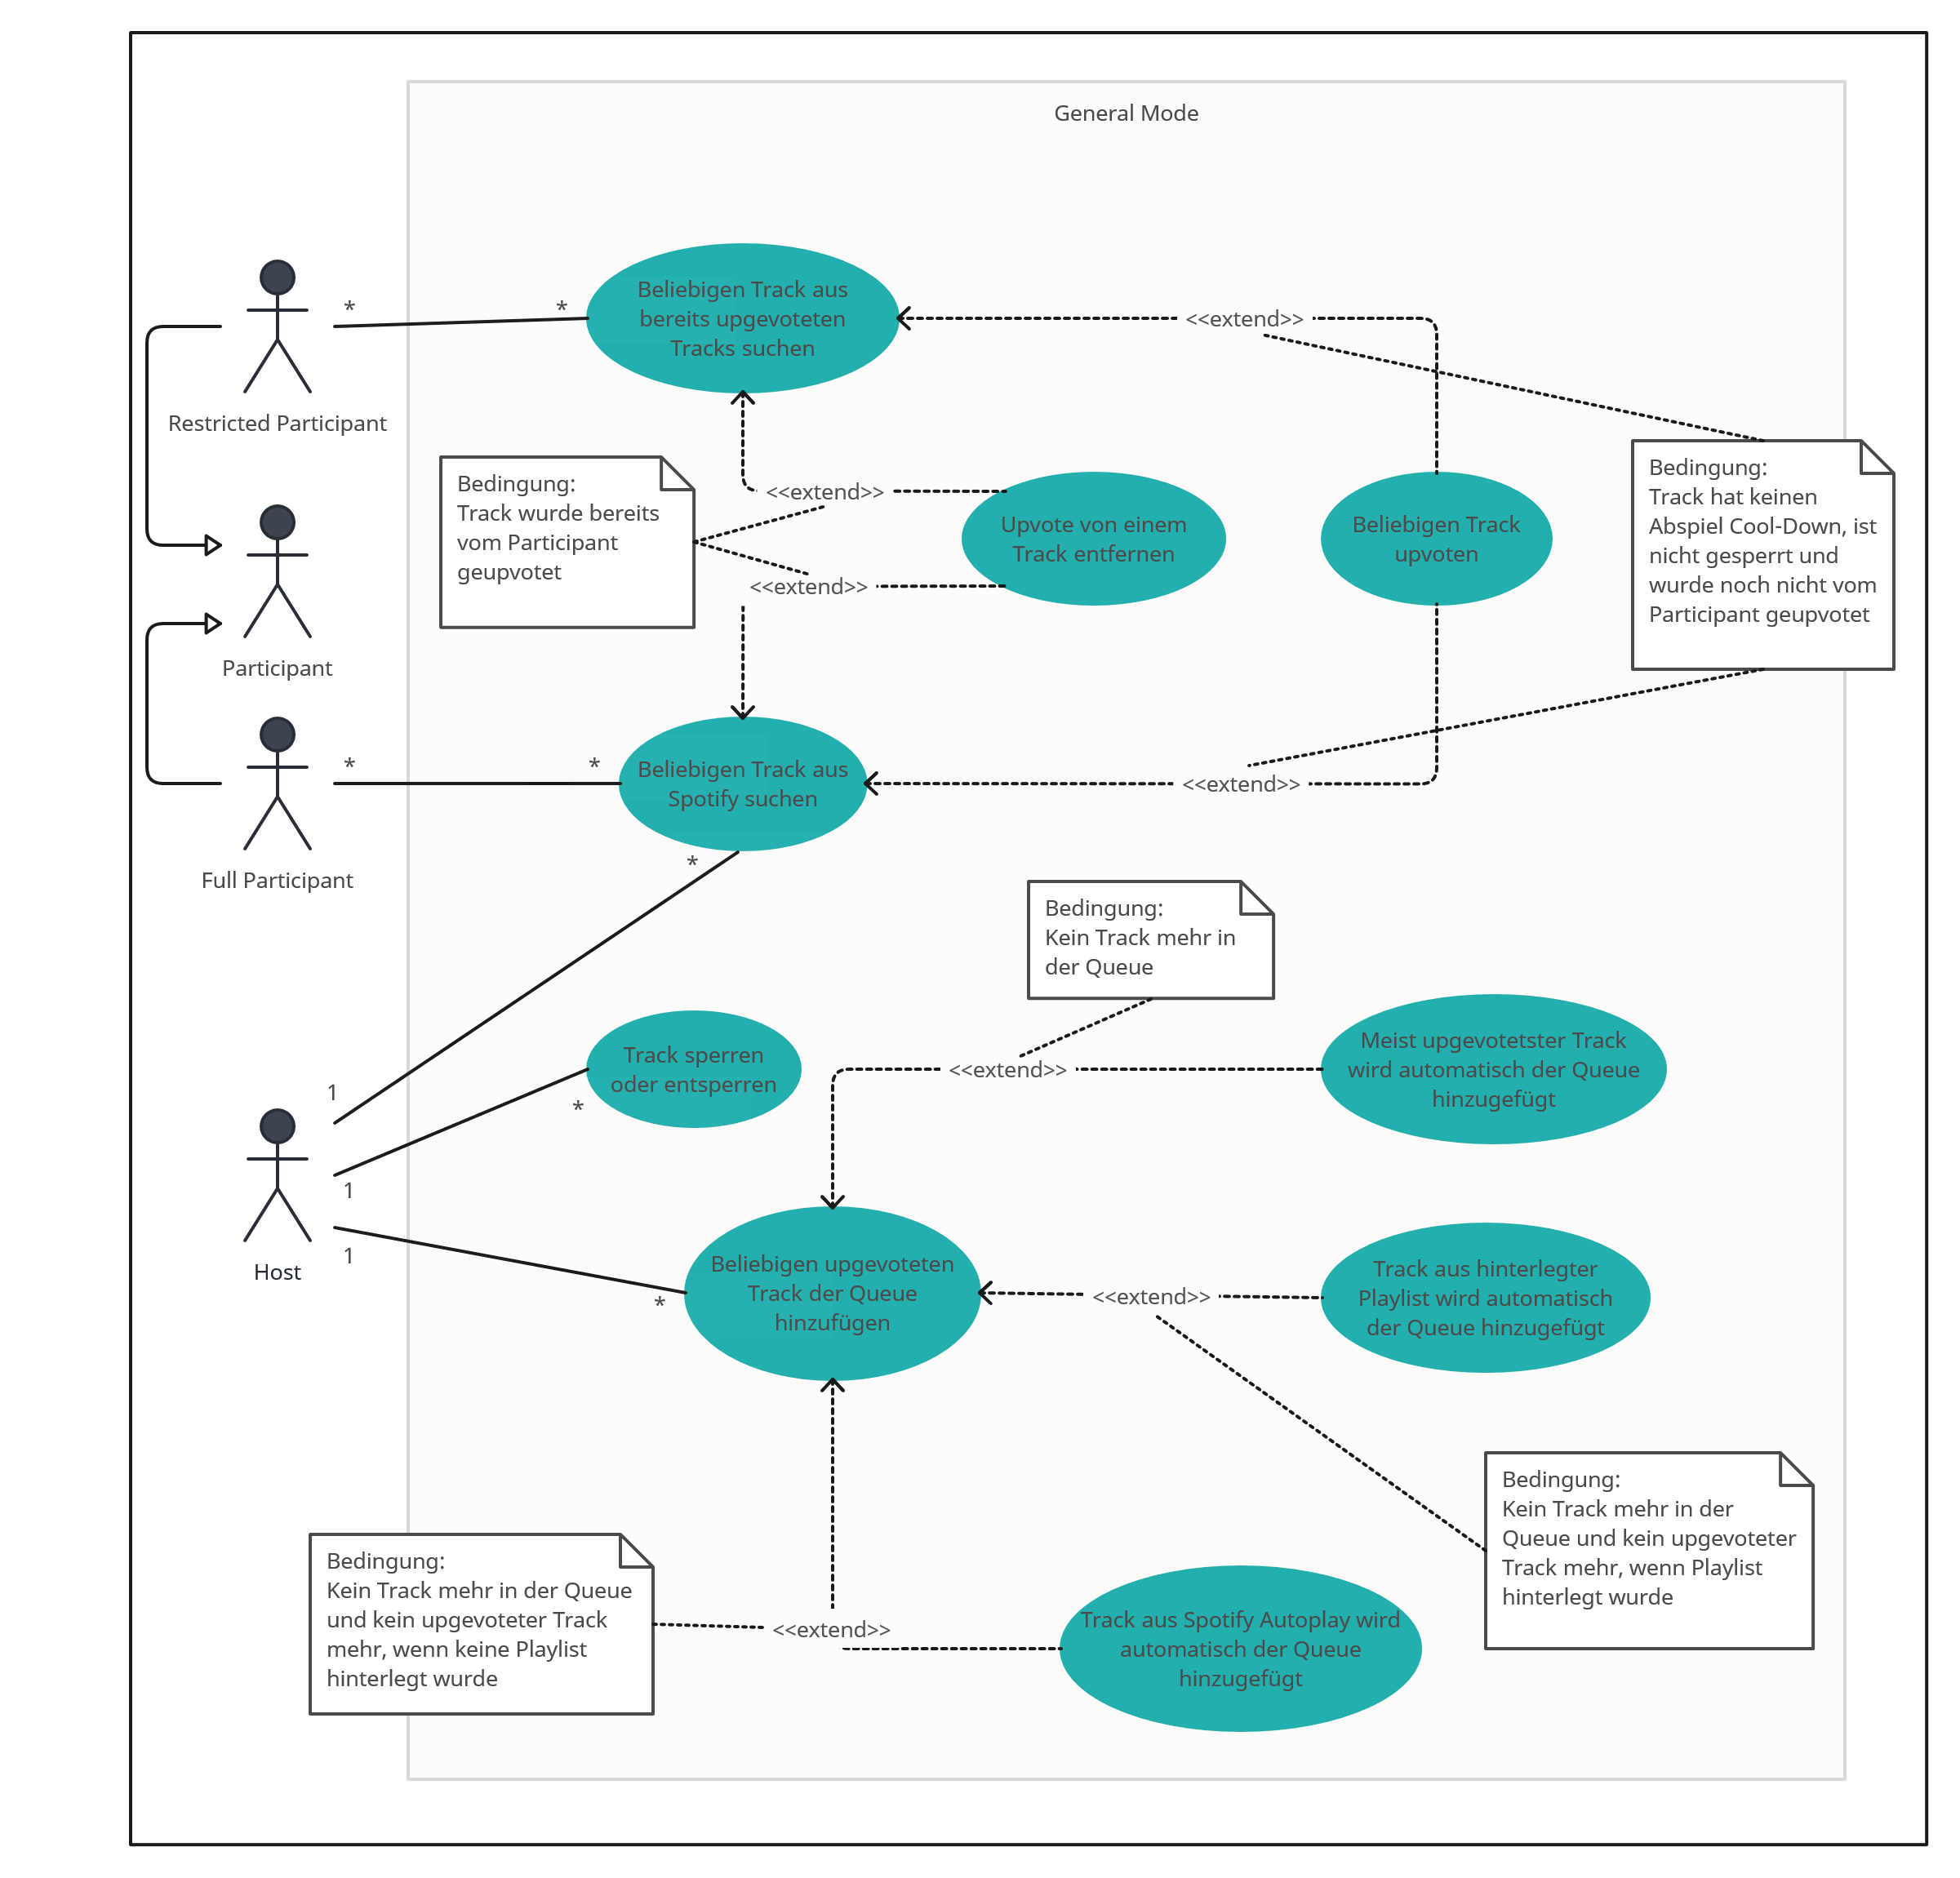
\includegraphics[width = 16cm]{LATEX/Pflichtenheft/GraphicDesigns/Use Case General Mode.png}
    \caption{General Mode}
    \label{fig:Use Case General Mode}
\end{figure}

\newpage

\section{Artist Mode}
\label{sec:Anwendungsfälle:Artist Mode}
\hypertarget{Artist Mode}{}

\begin{figure}[h]
    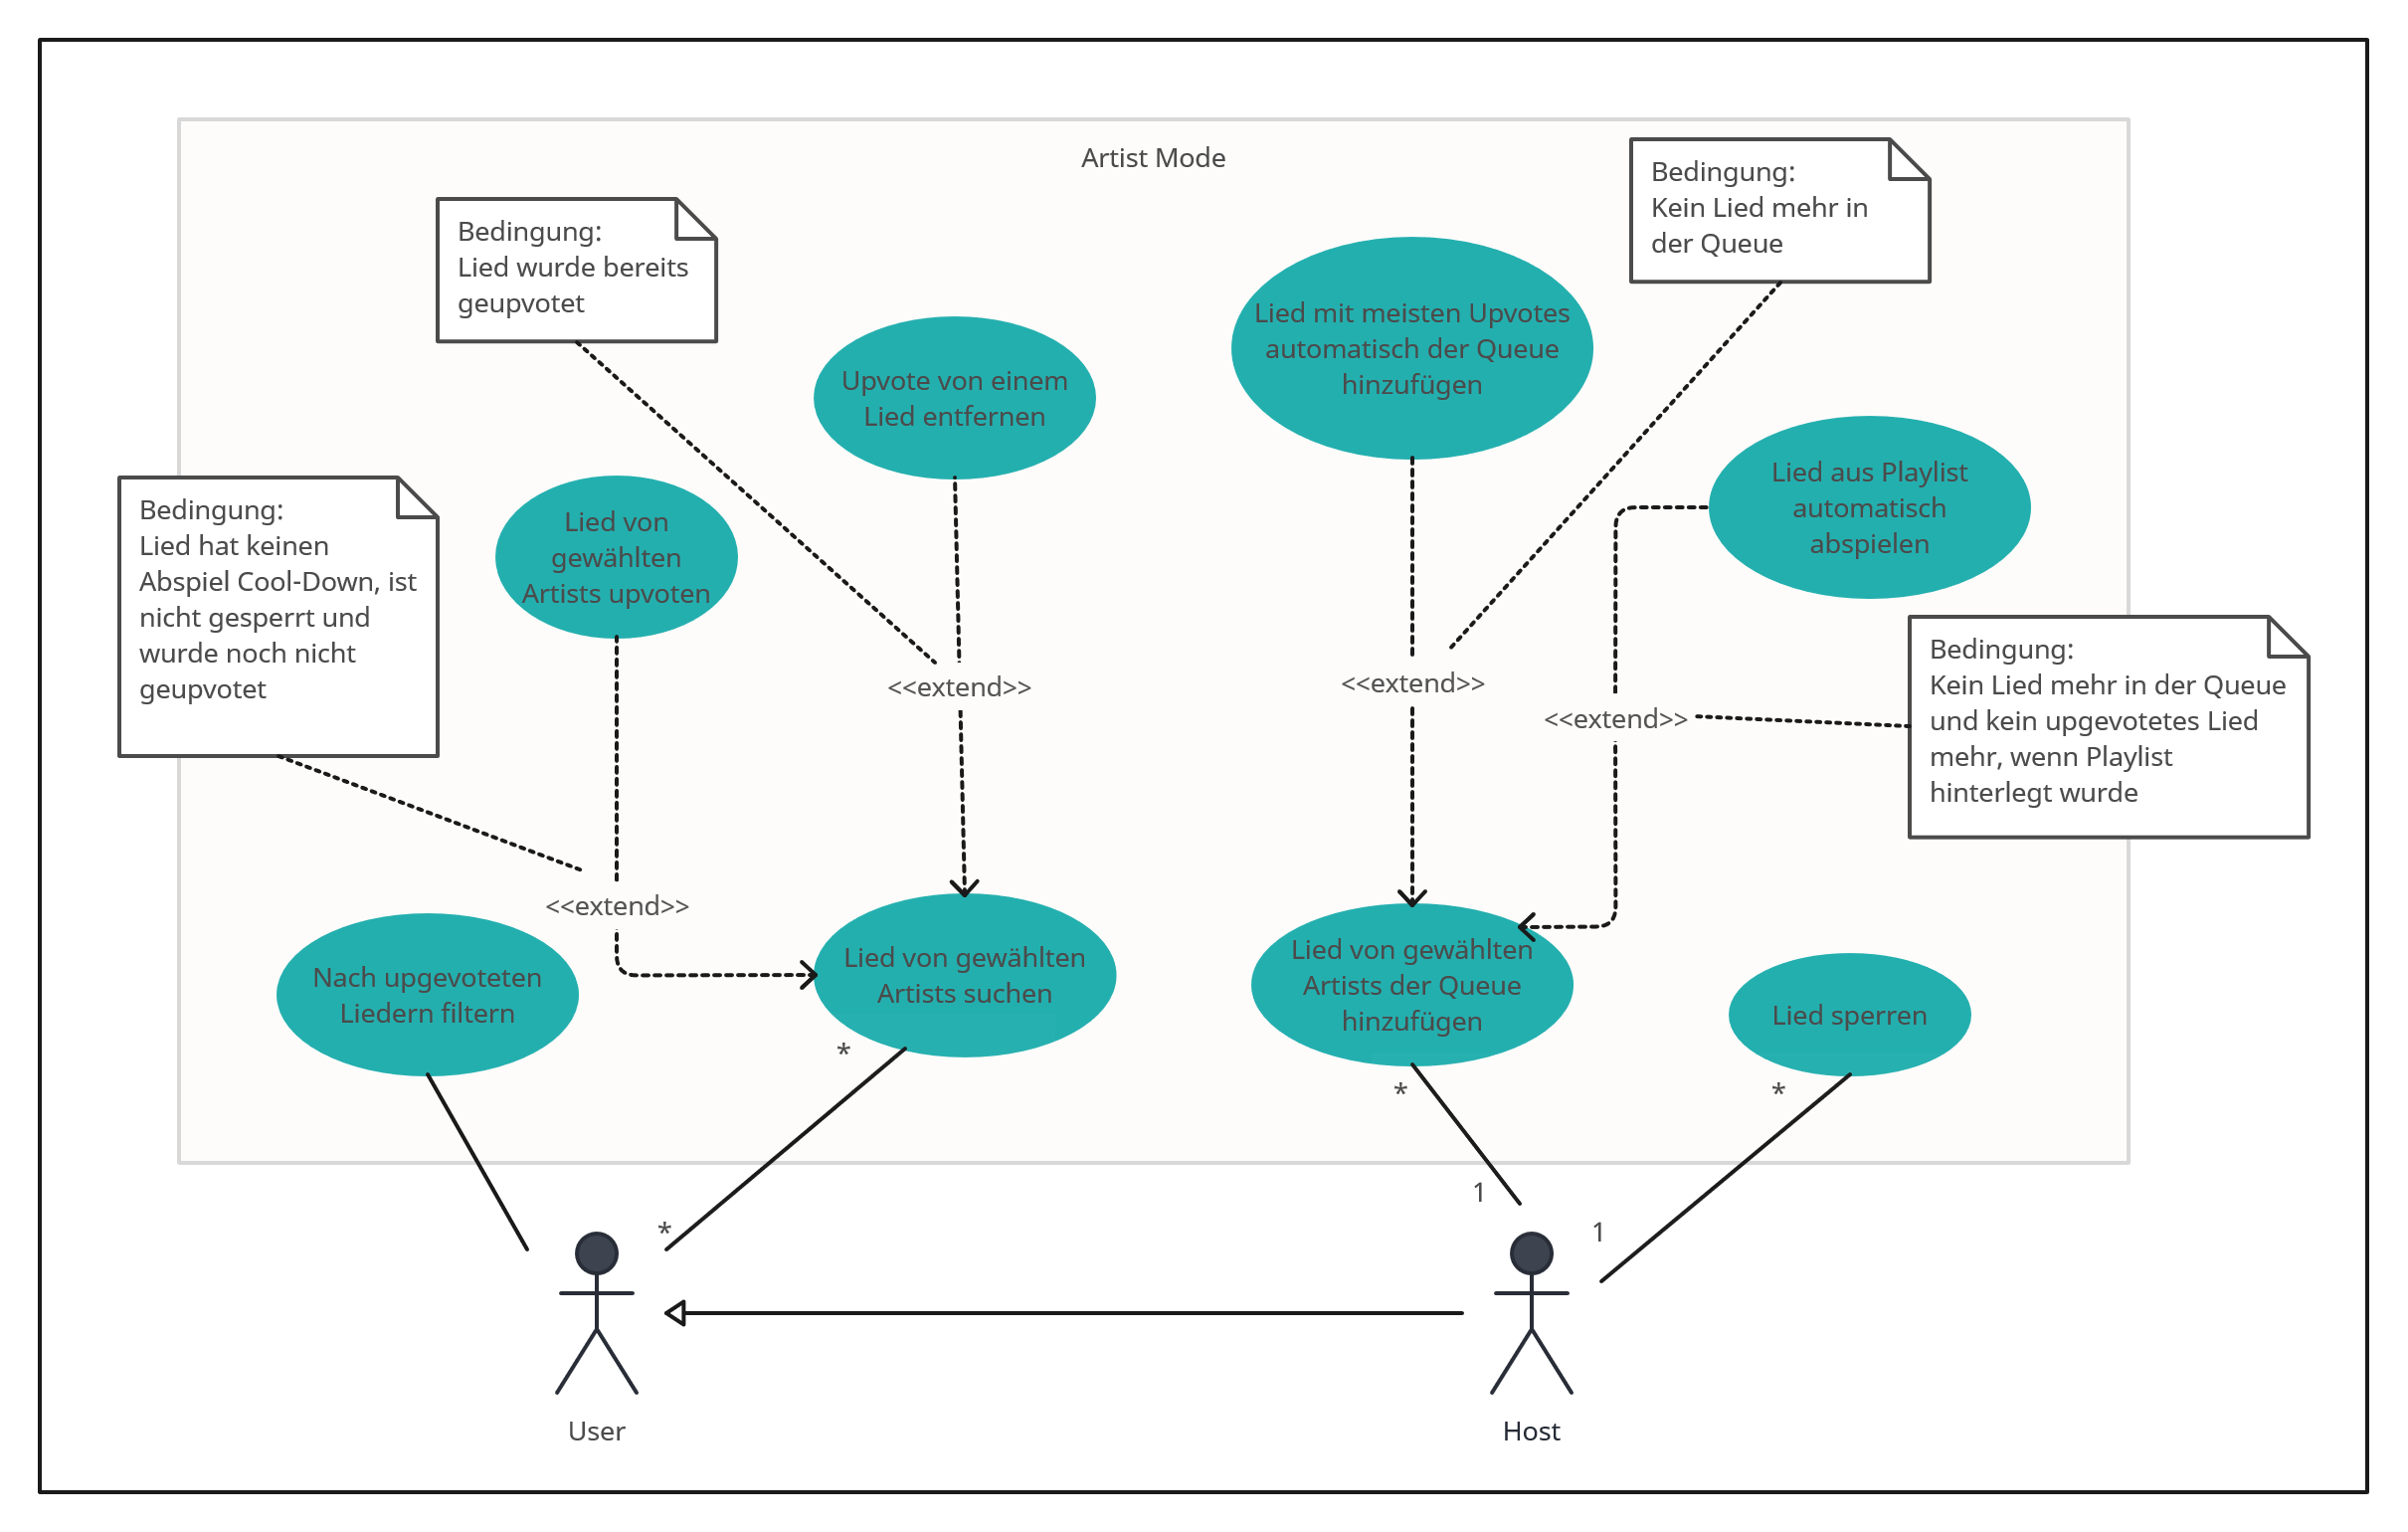
\includegraphics[width = 16cm]{LATEX/Pflichtenheft/GraphicDesigns/Use Case Artist Mode.png}
    \caption{Artist Mode}
    \label{fig:Use Case Artist Mode}
\end{figure}

\newpage

\section{Genre Mode}
\label{sec:Anwendungsfälle:Genre Mode}
\hypertarget{Genre Mode}{}

\begin{figure}[h]
    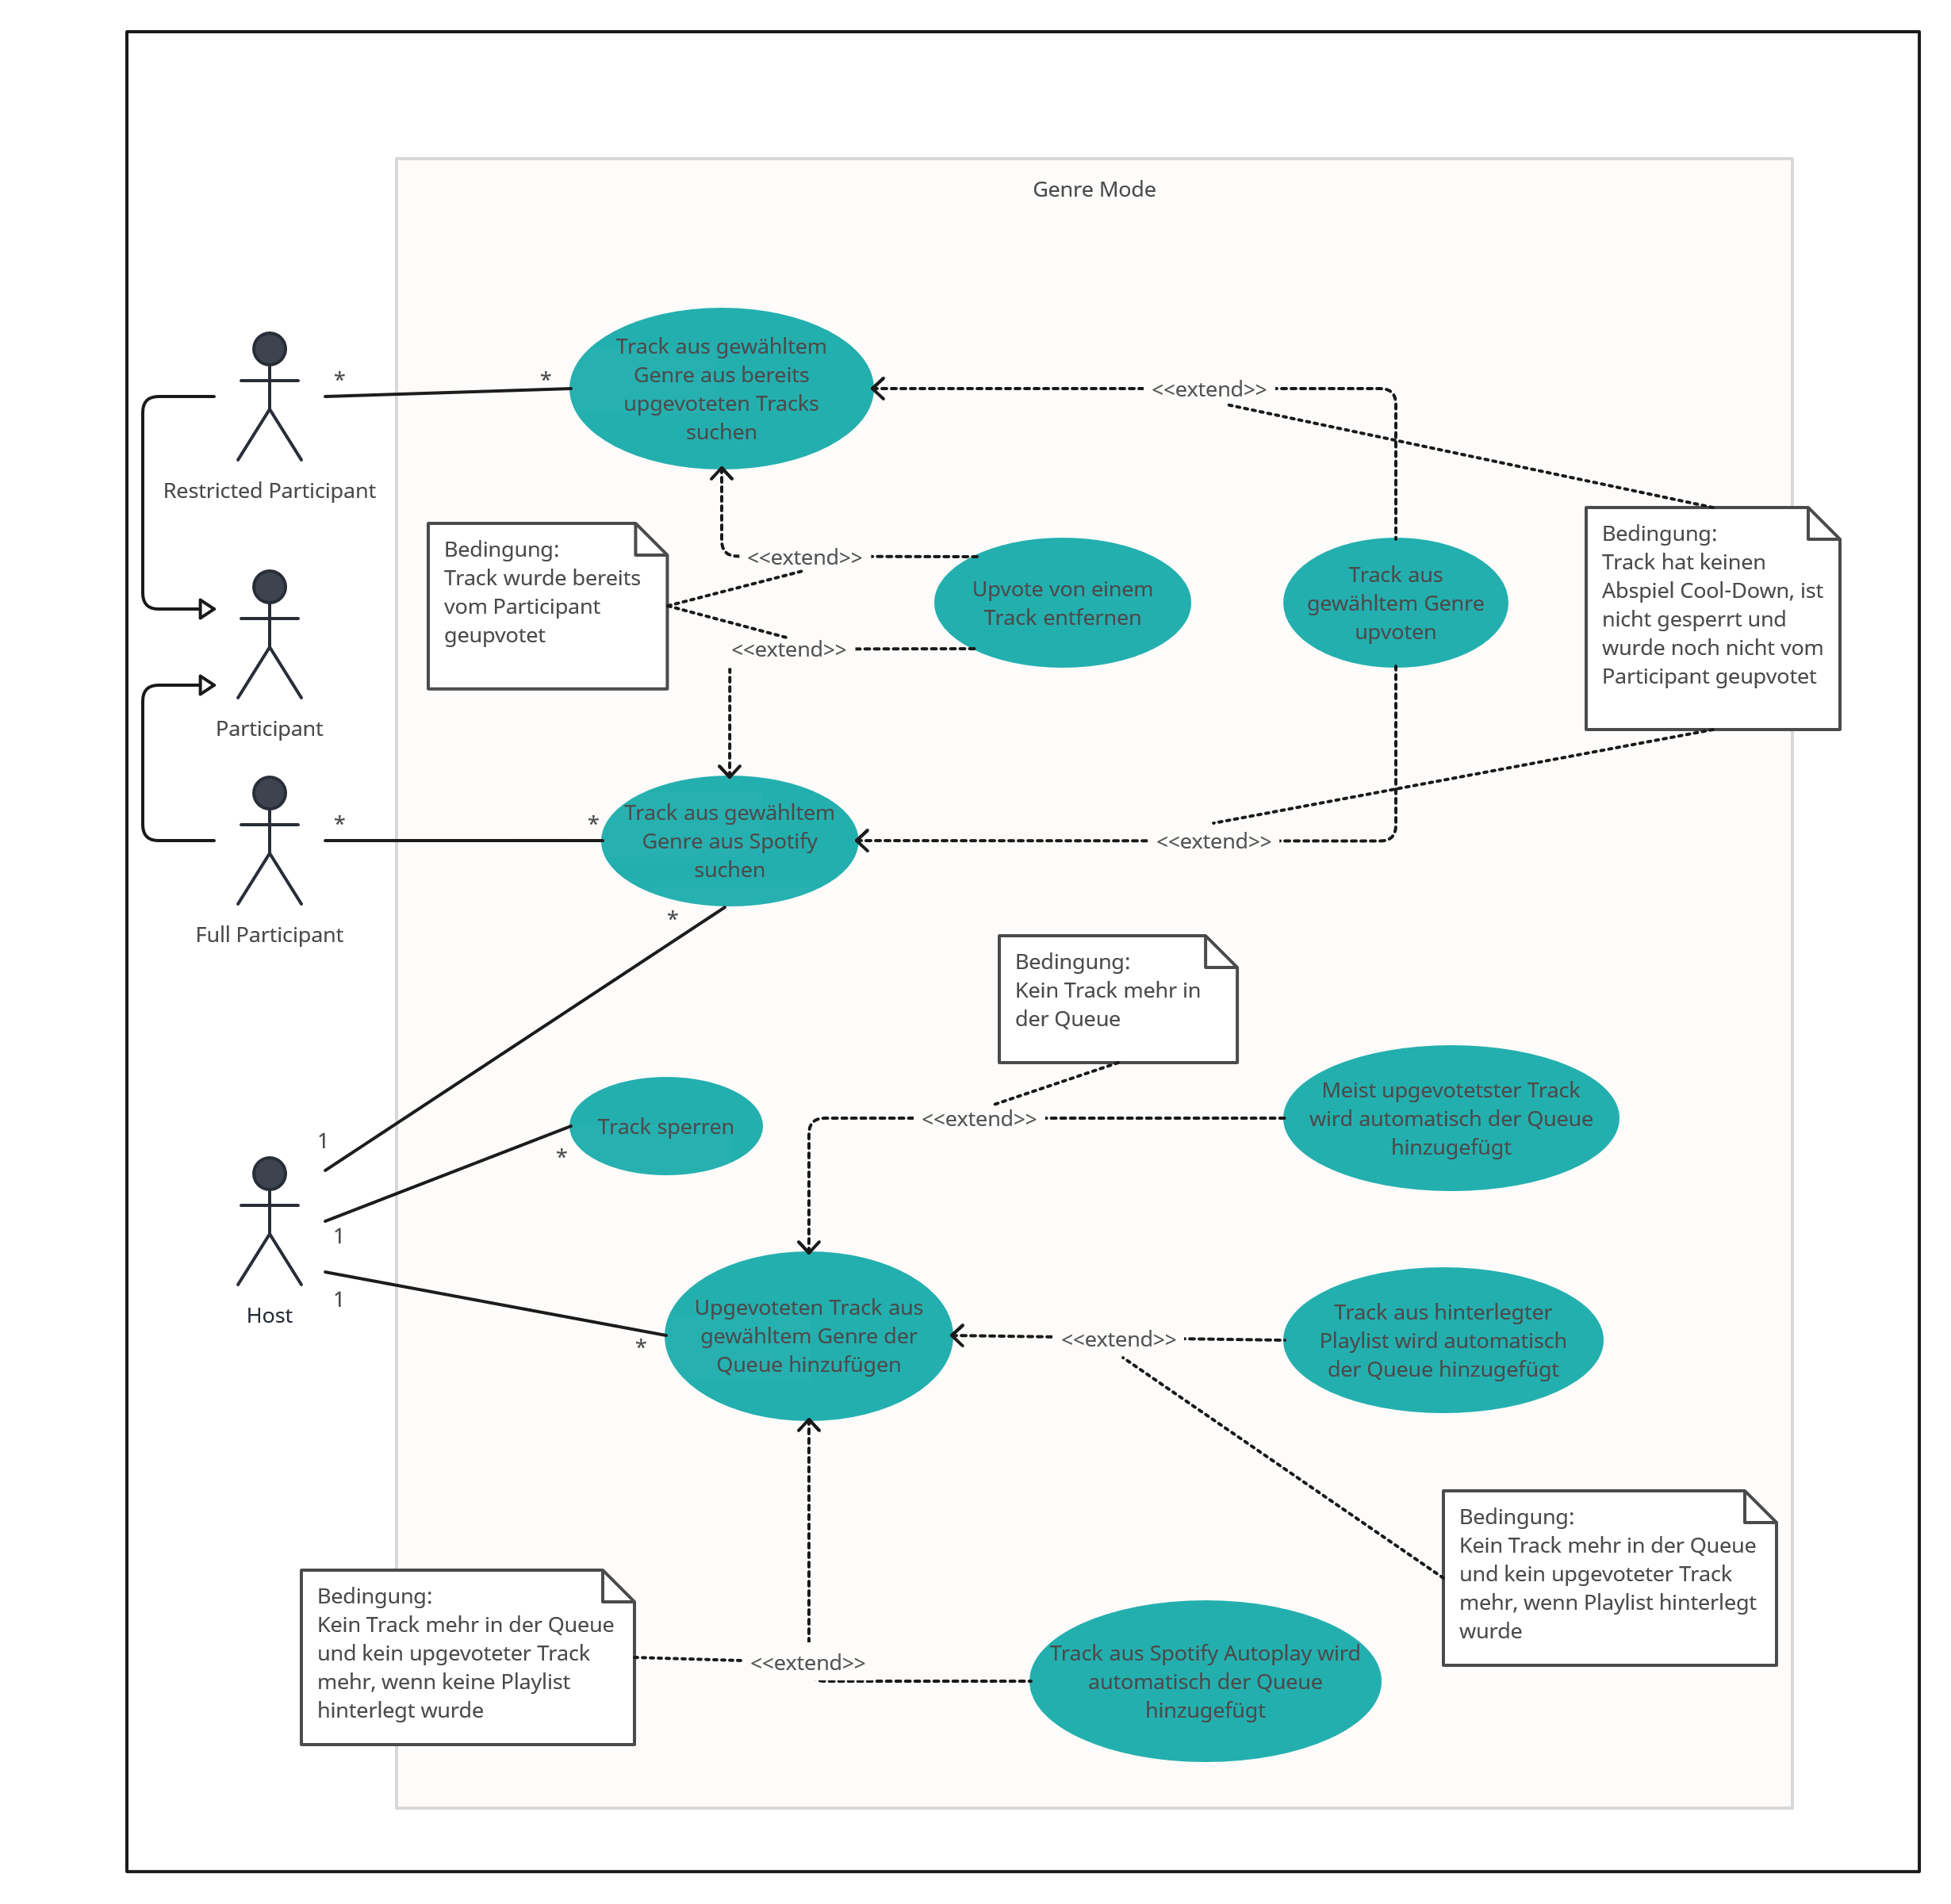
\includegraphics[width = 16cm]{LATEX/Pflichtenheft/GraphicDesigns/Use Case Genre Mode.png}
    \caption{Genre Mode}
    \label{fig:Use Case Genre Mode}
\end{figure}

\newpage

\section{Playlist Mode}
\label{sec:Anwendungsfälle:Playlist Mode}
\hypertarget{Playlist Mode}{}

\begin{figure}[h]
    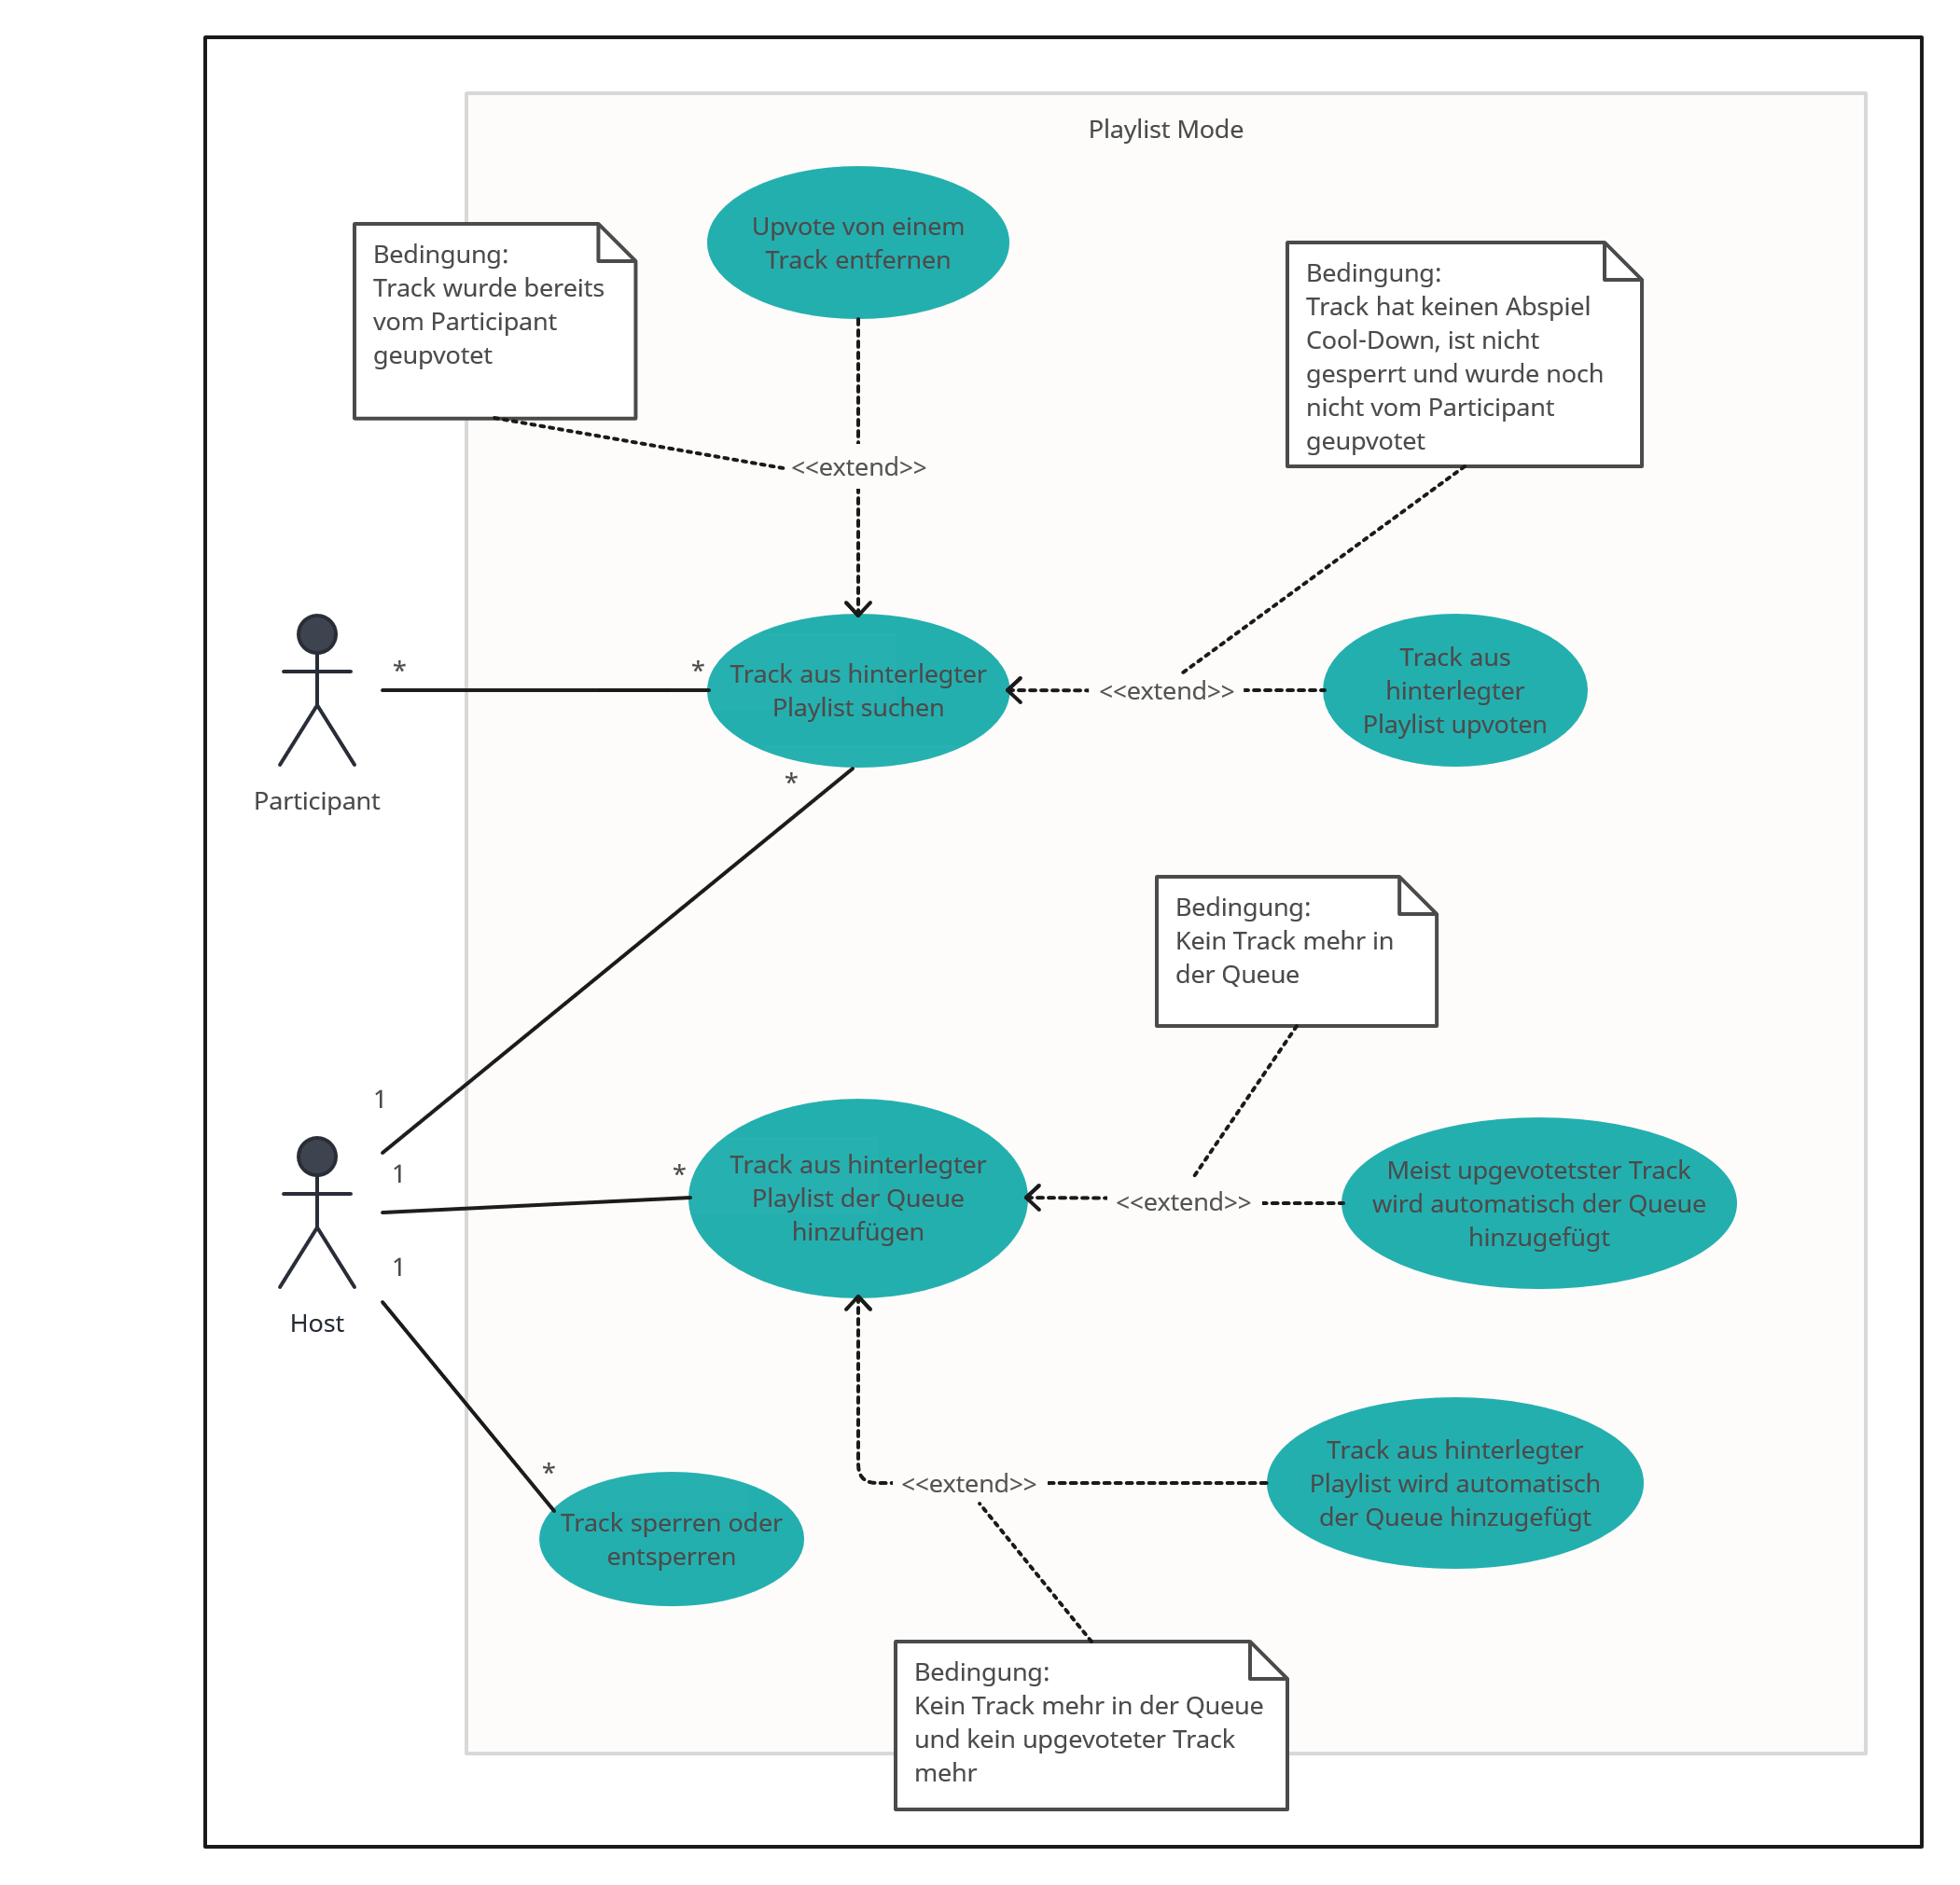
\includegraphics[width = 16cm]{LATEX/Pflichtenheft/GraphicDesigns/Use Case Playlist Mode.png}
    \caption{Playlist Mode}
    \label{fig:Use Case Playlist Mode}
\end{figure}



\chapter{Testfälle und -szenarien}
\label{chap:Tests}

In diesem Kapitel werden alle Testfälle und -szenarien definiert, die von einem oder mehreren Benutzer des Produkts durchgeführt werden können. Dabei wird das definierte Verhalten erwartet. Die hier definierten Testfälle sollen explizit keine detaillierten technischen Funktionalitäten auf technischer Ebene testen. Die Überprüfung solch detaillierter technischen Funktionalitäten wird durch Unittests abgedeckt, welche während der Entwurfs- und Implementierungsphase entworfen und implementiert werden.

\section{Testfälle}
\label{sec:Tests:Testfälle}

Die Testfälle lassen sich dem Kapitel Benutzeroberfläche und funktionale Anforderungen (Kapitel \ref{chap:Benutzeroberfläche}) entnehmen. Jede mit einer F-Nummer versehene funktionale Anforderung ist ein Testfall.

\section{Grundlegende Testszenarien}
\label{sec:Tests:GrundlegendeTestszenarien}
% do not show subsections in contents
\addtocontents{toc}{\protect\setcounter{tocdepth}{1}}

Grundlegende Testszenarien sind eine überschaubare und besonders essentielle Folge von Testfällen, die eine Benutzerinteraktion durchspielen. Sie setzen sich aus Testfällen oder bereits zuvor definierten grundlegenden Testszenarien zusammen.

\subsection{G1: Erstellen einer Session}
\label{subsec:Tests:GrundlegendeTestszenarien:G1}
\hypertarget{G1}{}
\newcommand{\gOne}{\hyperlink{G1}{G1: Erstellen einer Session }}
Ein mit Spotify-Premium verknüpfter User erstellt eine Session mit einem bestimmten Modus M und wird so zu ihrem Host. \\
\newcommand{\gNine}{\hyperlink{G9}{G9: Mit Spotify verknüpfen}}
Bereits abgelaufene Testszenarien: \gNine
\begin{itemize}
    \item \hyperlink{<F 101>}{<F 101>} Starten der App nach vollständiger Beendigung
    \item \hyperlink{<F 1.2>}{<F 1.2>} Beginnen der Sessionerstellung
    \item \hyperlink{<F 5.1.M>}{<F 5.1.M>} Wahl des Modus
    \item \hyperlink{<F 5.2>}{<F 5.2>} Bestätigen des Modus
    \item \hyperlink{<F 6.1>}{<F 6.1>}, \hyperlink{<F 6.2>}{<F 6.2>}/\hyperlink{<F 6.3>}{<F 6.3>}, \hyperlink{<F 6.4>}{<F 6.4>} Wählen entsprechender gültiger Einstellungen
    \item \hyperlink{<F 6.5>}{<F 6.5>} Bestätigen und Beginn der Session
\end{itemize}


\subsection{G2: Beitritt einer Session als Full Participant}
\label{subsec:Tests:GrundlegendeTestszenarien:G2}
\hypertarget{G2}{}
\newcommand{\gTwo}{\hyperlink{G2}{G2: Beitritt einer Session als Full Participant }}
Ein User tritt als Full Participant einer Session mit einem bestimmten Modus bei, die von einem anderen User als Host erstellt wurde. \\
Bereits abgelaufene Testszenarien: \gOne und außerdem \gNine
\begin{itemize}
    \item \hyperlink{<F 101>}{<F 101>} Starten der App nach vollständiger Beendung
    \item \hyperlink{<F 1.1>}{<F 1.1>} Beginnen des Sessionbeitrittsvorgangs
    \item \hyperlink{<F 2.1>}{<F 2.1>} Eingabe des Zugangscodes zum Sessionbeitritt
    \item \hyperlink{<F 2.1>}{<F 2.1>} Bestätigung des Zugangscodes zum Sessionbeitritt
\end{itemize}


\subsection{G3: Beitritt einer Session als Restricted Participant }
\label{subsec:Tests:GrundlegendeTestszenarien:G3}
\hypertarget{G3}{}
\newcommand{\gThree}{\hyperlink{G3}{G3: Beitritt einer Session als Restricted Participant }}
Ein User, tritt als Restricted Participant einer Session mit einem bestimmten Modus bei, die von einem anderen User als Host erstellt wurde. \\
Bereits abgelaufene Testszenarien: \gOne
\begin{itemize}
    \item \hyperlink{<F 101>}{<F 101>} Starten der App nach vollständiger Beendung
    \item \hyperlink{<F 1.1>}{<F 1.1>} Beginnen des Sessionbeitrittsvorgangs
    \item \hyperlink{<F 2.1>}{<F 2.1>} Eingabe des Zugangscodes zum Sessionbeitritt
    \item \hyperlink{<F 2.2.A>}{<F 2.2.A>} Bestätigung des Zugangscodes zum Sessionbeitritt
\end{itemize}

\subsection{G4: Upvoten eines neuen Tracks als Full Participant }
\label{subsec:Tests:GrundlegendeTestszenarien:G4}
\hypertarget{G4}{}
\newcommand{\gFour}{\hyperlink{G4}{G4: Upvoten eines neuen Tracks als Full Participant }}
Ein User, der schon als Full Particpant einer Session mit einem bestimmten Modus beigetreten ist, die von einem anderen User als Host erstellt wurde, votet einen neuen Track up. \\
Bereits abgelaufene Testszenarien: \gTwo
\begin{itemize}
    \item \hyperlink{<F 3.4>}{<F 3.4>} Öffnen der Tracksuche
    \item \hyperlink{<F 4.3>}{<F 4.3>} Suchen eines Tracks
    \item \hyperlink{<F 4.4.A>}{<F 4.4.A>} Upvoten des Tracks
\end{itemize}

\subsection{G5: Upvoten eines neuen Tracks als Host}
\label{subsec:Tests:GrundlegendeTestszenarien:G5}
\hypertarget{G5}{}
\newcommand{\gFive}{\hyperlink{G5}{G5: Upvoten eines neuen Tracks als Host }}
Der Host votet einen neuen Track up. \\
Bereits abgelaufene Testszenarien: \gOne
\begin{itemize}
    \item \hyperlink{<F 7.9>}{<F 7.9>} Öffnen der Tracksuche
    \item \hyperlink{<F 8.3>}{<F 8.3>} Suchen eines Tracks
    \item \hyperlink{<F 8.3>}{<F 8.3>} Upvoten des Tracks
\end{itemize}

\subsection{G6: Upvoten eines Tracks}
\label{subsec:Tests:GrundlegendeTestszenarien:G6}
\hypertarget{G6}{}
\newcommand{\gSix}{\hyperlink{G6}{G6: Upvoten eines Tracks }}
Ein Participant einer Session mit einem bestimmten Modus votet einen Track aus der Vorschlagsliste up. \\
Bereits abgelaufene Testszenarien: \gFour, optional \gThree
\begin{itemize}
    \item \hyperlink{<F 3.3.A>}{<F 3.3.A>} Upvote für einen Track
\end{itemize}

\subsection{G7: Hinzufügen eines Tracks aus der Vorschlagsliste zur Queue}
\label{subsec:Tests:GrundlegendeTestszenarien:G7}
\hypertarget{G7}{}
\newcommand{\gSeven}{\hyperlink{G7}{G7: Hinzufügen eines Tracks aus der Vorschlagsliste zur Queue }}
Der Host fügt einen bestimmten Track aus der Vorschlagsliste zur Queue hinzu, sodass dieser in Zukunft abgespielt wird. \\
Bereits abgelaufene Testszenarien: \gOne
\begin{itemize}
    \item \hyperlink{<F7.7>}{<F7.7>}, \hyperlink{<F 7.7.A>}{<F 7.7.A>} Einfügen eines Tracks aus der Vorschlagsliste in die Queue
\end{itemize}

\subsection{G8: Vollständiges Beenden einer Session}
\label{subsec:Tests:GrundlegendeTestszenarien:G8}
\hypertarget{G8}{}
\newcommand{\gEight}{\hyperlink{G8}{G8: Vollständiges Beenden einer Session }}
Alle Participants verlassen die Session, anschließend beendet der Host die Session. Alle User verlassen und beenden die App. \\
Bereits abgelaufene Testszenarien: Mindestens \gOne, optional mehrfach \gTwo oder \gThree
\begin{itemize}
    \item Alle Participants der Session: \hyperlink{<F 3.5>}{<F 3.5>}, <F 3.5.A> Verlassen der Session
    \item \hyperlink{<F 7.10>}{<F 7.10>}, \hyperlink{<F 7.10.A>}{<F 7.10.A>} Löschen der Session (Host)
    \item Alle User (Participants und Host): \hyperlink{<F 100>}{<F 100>} Vollständiges Beenden der App
\end{itemize}


\subsection{G9: Mit Spotify verknüpfen}
\label{subsec:Tests:GrundlegendeTestszenarien:G9}
\hypertarget{G9}{}
\renewcommand{\gNine}{\hyperlink{G9}{G9: Mit Spotify verknüpfen }}
Ein User verknüpft sich nach dem Start der App mit Spotify. \\
Bereits abgelaufene Testszenarien: -
\begin{itemize}
    \item \hyperlink{<F 101>}{<F 101>} Starten der App nach vollständiger Beendung
    \item \hyperlink{<F 1.3.A>}{<F 1.3.A>} Mit Spotify verknüpfen
\end{itemize}


\subsection{G10: Verwenden der Session-Info als Participant}
\label{subsec:Tests:GrundlegendeTestszenarien:G10}
\hypertarget{G10}{}
\newcommand{\gTen}{\hyperlink{G10}{G10: Verwenden der Session-Info als Participant }}
Ein Participant öffnet die Session-Info in der \hyperlink{sessionVoteView}{sessionVoteView (A 3.3)}, teilt den Beitrittslink und schließt die Session-Info wieder. \\
Bereits abgelaufene Testszenarien: \gTwo oder \gThree
\begin{itemize}
    \item \hyperlink{<F 3.1>}{<F 3.1>} Öffnen der Session-Info
    \item \hyperlink{<F 9.1>}{<F 9.1>} Teilen der Beitrittslinks
    \item \hyperlink{<F 9.2>}{<F 9.2>} Schließen der Session-Info
\end{itemize}


\subsection{G11: Verwenden der Statistiken als Participant}
\label{subsec:Tests:GrundlegendeTestszenarien:G11}
\hypertarget{G11}{}
\newcommand{\gEleven}{\hyperlink{G11}{G11: Verwenden der Statistiken als Participant }}
Ein Participant öffnet die Statistiken in der \hyperlink{sessionVoteView}{sessionVoteView (A 3.3)}, teilt das Statistik-Bild und schließt die Statistiken wieder. \\
Bereits abgelaufene Testszenarien: \gTwo oder \gThree
\begin{itemize}
    \item \hyperlink{<F 3.2>}{<F 3.2>} Öffnen der Statistiken
    \item \hyperlink{<F 10.1>}{<F 10.1>} Teilen des Statistik-Bilds
    \item \hyperlink{<F 10.2>}{<F 10.2>} Schließen der Statistiken
\end{itemize}


\subsection{G12: Upvote von Track entfernen}
\label{subsec:Tests:GrundlegendeTestszenarien:G12}
\hypertarget{G12}{}
\newcommand{\gTwelve}{\hyperlink{G12}{G12: Upvote von Track entfernen }}
Ein Participant einer Session entfernt sein Upvote wieder von einem Track. \\
Bereits abgelaufene Testszenarien: \gSix
\begin{itemize}
    \item \hyperlink{<F 3.3.B>}{<F 3.3.B>} Upvote von einen Track entfernen
\end{itemize}

\subsection{G13: Erstellen einer Session im Artist Mode}
\label{subsec:Tests:GrundlegendeTestszenarien:G13}
\hypertarget{G13}{}
\newcommand{\gThirteen}{\hyperlink{G13}{G13: Erstellen einer Session im Artist Mode }}
Ein mit Spotify-Premium verknüpfter User eröffnet eine Session im Artist Mode. \\
Bereits abgelaufene Testszenarien: \gNine
\begin{itemize}
    \item \hyperlink{<F 101>}{<F 101>} Starten der App nach vollständiger Beendung
    \item \hyperlink{<F 1.2>}{<F 1.2>} Beginnen der Sessionerstellung
    \item \hyperlink{<F 5.1.2>}{<F 5.1.2>} Wahl des Artist Mode
    \item \hyperlink{<F 5.2>}{<F 5.2>} Bestätigen des Modus
    \item \hyperlink{<F 6.2.A>}{<F 6.2.A>} Öffnen der Artist-Suche
    \item \hyperlink{<F 11.1>}{<F 11.1>} Suchen nach einem Artist
    \item \hyperlink{<F 11.2.A>}{<F 11.2.A>} (3x) Hinzufügen der ersten drei Artists
    \item \hyperlink{<F 11.2.B>}{<F 11.2.B>} Entfernen des ersten Artists
    \item \hyperlink{<F 11.3>}{<F 11.3>} Verlassen der Artist-Suche
    \item \hyperlink{<F 6.3.A>}{<F 6.3.A>} Entfernen des ersten Artists
    \item \hyperlink{<F 6.5>}{<F 6.5>} Bestätigen der Moduseinstellungen
\end{itemize}


\subsection{G14: Erstellen einer Session im Genre Mode}
\label{subsec:Tests:GrundlegendeTestszenarien:G14}
\hypertarget{G14}{}
\newcommand{\gFourteen}{\hyperlink{G14}{G14: Erstellen einer Session im Genre Mode }}
Ein mit Spotify-Premium verknüpfter User eröffnet eine Session im Genre Mode. \\
Bereits abgelaufene Testszenarien: \gNine
\begin{itemize}
    \item \hyperlink{<F 101>}{<F 101>} Starten der App nach vollständiger Beendung
    \item \hyperlink{<F 1.2>}{<F 1.2>} Beginnen der Sessionerstellung
    \item \hyperlink{<F 5.1.3>}{<F 5.1.3>} Wahl des Genre Mode
    \item \hyperlink{<F 5.2>}{<F 5.2>} Bestätigen des Modus
    \item \hyperlink{<F 6.2.B>}{<F 6.2.B>} Öffnen der Genre-Suche
    \item \hyperlink{<F 12.1>}{<F 12.1>} Suchen nach einem Genre
    \item \hyperlink{<F 12.2.A>}{<F 12.2.A>} (3x) Hinzufügen der ersten drei Genres
    \item \hyperlink{<F 12.2.B>}{<F 12.2.B>} Entfernen des ersten Genres
    \item \hyperlink{<F 12.3>}{<F 12.3>} Verlassen der Genre-Suche
    \item \hyperlink{<F 6.3.B>}{<F 6.3.B>} Entfernen des ersten Genres
    \item \hyperlink{<F 6.5>}{<F 6.5>} Bestätigen der Moduseinstellungen
\end{itemize}


\addtocontents{toc}{\protect\setcounter{tocdepth}{2}}
\section{Erweiterte Testszenarien}
\label{sec:Tests:ErweiterteTestszenarien}
\addtocontents{toc}{\protect\setcounter{tocdepth}{1}}

Erweiterte Testszenarien sind eine nicht-essentielle und möglicherweise längere Folge von atomaren Testfällen, die eine Benutzerinteraktion durchspielen. Sie setzen sich aus Testfällen und grundlegenden Testszenarien zusammen.


\subsection{E1: Grundlegende Session-Funktionalität}
\label{subsec:Tests:ErweiterteTestszenarien:E1}
Ein Host (H) erstellt eine Session, in welche ein Full Participant (FP) beitritt. Anschließend wird die Session ordnungsgemäß beendet und alle User beenden die App.
\begin{itemize}
    \item \gOne (H)
    \item \gTwo (FP)
    \item \gEight
\end{itemize}


\subsection{E2: Track-Upvote und Abspielen}
\label{subsec:Tests:ErweiterteTestszenarien:E1}
Ein Host (H) erstellt eine Session, in welche ein Full Participant (FP) und ein Restricted Partipant (RP) beitreten. FP schlägt einen Song vor durch Upvote, den auch RP upvotet und H dann in die Queue hinzufügt.
\begin{itemize}
    \item \gOne (H)
    \item \gTwo (FP)
    \item \gThree (RP)
    \item \gFour (FP)
    \item \gSix (RP)
    \item \gSeven (H)
\end{itemize}


\subsection{E3: Abspielen von fünf vorgeschlagenen zufälligen Tracks}
\label{subsec:Tests:ErweiterteTestszenarien:E3}
Ein Host (H) erstellt eine Session, in welche ein Full Participant (FP) und zwei Restricted Partipants (RP1 und RP2) beitreten. H schlägt zwei Tracks vor, FP schlägt drei Tracks vor. RP1 votet einen Track von H und einen Track von FP up. RP2 votet nur denselben Track von H up. H votet einen Track up und entfernt sein Upvote wieder. H spielt die Tracks nach Anzahl der Upvotes ab. Die Tracks sind zufällig gewählt, der Test ist randomisiert.
\begin{itemize}
    \item \gOne (H)
    \item \gTwo (FP)
    \item \gThree (RP1)
    \item \gThree (RP2)
    \item \gFive (H) (2x)
    \item \gFour (FP) (3x)
    \item \gSix, Track von H (RP1)
    \item \gSix, Track von FP (RP1)
    \item \gSix, selber Track von H (RP2)
    \item \hyperlink{<F 7.6.A>}{<F 7.6.A>} Upvoten des ersten Tracks aus der Vorschlagsliste
    \item \hyperlink{<F 7.6.B>}{<F 7.6.B>} Entfernen des Upvote vom ersten Track aus der Vorschlagsliste
    \item \gSeven (H) (5x, in beliebiger Reihenfolge)
\end{itemize}


\subsection{E4: Testen aller Navigations-Buttons}
\label{subsec:Tests:ErweiterteTestszenarien:E4}
Ein mit Spotify-Premium verknüpfter User testet alle Navigations-Buttons, die es in der App gibt. Der User ist erst in der Rolle eines Participants, indem er einer bereits mit dem Testszenario \gOne erstellten Session beitritt. Danach ist er in der Rolle des Hosts.
\begin{itemize}
    \item In der Participant-Rolle:
    \item \gNine
    \item \hyperlink{<F 1.1>}{<F 1.1>} Beginnen des Sessionbeitrittsvorgangs
    \item \hyperlink{<F 2.3>}{<F 2.3>} Öffnen des QR-Code-Readers (ohne Scannen eines QR-Codes)
    \item \hyperlink{<F 2.4>}{<F 2.4>} Schließen des QR-Code-Readers
    \item \hyperlink{<F 2.5>}{<F 2.5>} Verlassen des Sessionbeitrittsvorgangs
    \item \gTwo
    \item \hyperlink{<F 3.4>}{<F 3.4>} Öffnen der Tracksuche
    \item \hyperlink{<F 4.1>}{<F 4.1>} Öffnen der Session-Info
    \item \hyperlink{<F 9.2>}{<F 9.2>} Schließen der Session-Info
    \item \hyperlink{<F 4.2>}{<F 4.2>} Öffnen der Statistiken
    \item \hyperlink{<F 10.2>}{<F 10.2>} Schließen der Statistiken
    \item \hyperlink{<F 4.5>}{<F 4.5>} Verlassen der Tracksuche
    \item \gTen
    \item \gEleven
    \item \hyperlink{<F 3.5>}{<F 3.5>}, \hyperlink{<F3.5.B}{<F3.5.B}> Verlassen der Session, aber keine Bestätigung
    \item \hyperlink{<F 3.5>}{<F 3.5>}, \hyperlink{<F3.5.A>}{<F3.5.A>} Verlassen der Session (mit Bestätigung)
    \item \hyperlink{<F 10.2>}{<F 10.2>} Schließen der Statistiken
    \item In der Host-Rolle:
    \item \hyperlink{<F 1.2>}{<F 1.2>} Beginn der Moduswahl
    \item \hyperlink{<F 5.3>}{<F 5.3>} Verlassen der Moduswahl
    \item \hyperlink{<F 1.2>}{<F 1.2>} Beginn der Moduswahl
    \item \hyperlink{<F 5.2>}{<F 5.2>} Bestätigen des Modus
    \item \hyperlink{<F 6.6>}{<F 6.6>} Velassen der Moduseinstellungen
    \item \hyperlink{<F 5.2>}{<F 5.2>} Bestätigen des Modus
    \item \hyperlink{<F 6.5>}{<F 6.5>} Bestätigen der Moduseinstellungen
    \item \hyperlink{<F 7.1>}{<F 7.1>} Öffnen der Session-Info
    \item \hyperlink{<F 9.2>}{<F 9.2>} Schließen der Session-Info
    \item \hyperlink{<F 7.2>}{<F 7.2>} Öffnen der Statistiken
    \item \hyperlink{<F 10.2>}{<F 10.2>} Schließen der Statistiken
    \item \hyperlink{<F 7.9>}{<F 7.9>} Öffnen der Tracksuche
    \item \hyperlink{<F 8.1>}{<F 8.1>} Öffnen der Session-Info
    \item \hyperlink{<F 9.2>}{<F 9.2>} Schließen der Session-Info
    \item \hyperlink{<F 8.2>}{<F 8.2>} Öffnen der Statistiken
    \item \hyperlink{<F 10.2>}{<F 10.2>} Schließen der Statistiken
    \item \hyperlink{<F 8.6>}{<F 8.6>} Verlassen der Tracksuche
    \item \hyperlink{<F 7.10>}{<F 7.10>}, \hyperlink{<F 7.10.B>}{<F 7.10.B>} Beenden der Session, aber keine Bestätigung
    \item \hyperlink{<F 7.10>}{<F 7.10>}, \hyperlink{<F 7.10.A>}{<F 7.10.A>} Beenden der Session (mit Bestätigung)
    \item \hyperlink{<F 10.2>}{<F 10.2>} Schließen der Statistiken
    \item \gThirteen
    \item \hyperlink{<F 7.10>}{<F 7.10>}, \hyperlink{<F 7.10.A>}{<F 7.10.A>} Beenden der Session (mit Bestätigung)
    \item \hyperlink{<F 10.2>}{<F 10.2>} Schließen der Statistiken
    \item \gFourteen
    \item \hyperlink{<F 7.10>}{<F 7.10>}, \hyperlink{<F 7.10.A>}{<F 7.10.A>} Beenden der Session (mit Bestätigung)
    \item \hyperlink{<F 10.2>}{<F 10.2>} Schließen der Statistiken
    \item \hyperlink{<F 1.4>}{<F 1.4>}, \hyperlink{<F 1.4.B>}{<F 1.4.B>}  Beenden der App, aber keine Bestätigung
    \item \hyperlink{<F 1.4>}{<F 1.4>}, \hyperlink{<F 1.4.A>}{<F 1.4.A>} Beenden der App (mit Bestätigung)
\end{itemize}


\subsection{E5: Testen fast aller Host-Funktionalitäten}
\label{subsec:Tests:ErweiterteTestszenarien:E5}
Ein mit Spotify-Premium verknüpfter User öffnet eine Session und testet fast alle Funktionalitäten, die ihm als Host dieser Session durch die Kontrollansicht zur Verfügung stehen.
\begin{itemize}
    \item \gOne
    \item \hyperlink{<F 7.9>}{<F 7.9>} Öffnen der Tracksuche
    \item \hyperlink{<F 8.3>}{<F 8.3>} Suchen nach einem Track
    \item \hyperlink{<F 8.4.A>}{<F 8.4.A>} (3x) Upvoten der ersten drei Tracks
    \item \hyperlink{<F 8.4.B>}{<F 8.4.B>} Entfernen des Upvote vom letzten der drei Tracks
    \item \hyperlink{<F 8.5>}{<F 8.5>} , \hyperlink{<F 8.5.A>}{<F 8.5.A>} (2x) Hinzufügen des vierten und fünften Tracks zur Queue
    \item \hyperlink{<F 8.5>}{<F 8.5>} , \hyperlink{<F 8.5.B>}{<F 8.5.B>} Sperren des sechsten Tracks
    \item \hyperlink{<F 8.5>}{<F 8.5>} , \hyperlink{<F 8.5.B>}{<F 8.5.B>} Entsperren des sechsten Tracks
    \item \hyperlink{<F 8.6>}{<F 8.6>} Verlassen der Tracksuche
    \item \hyperlink{<F 7.3.A>}{<F 7.3.A>} Upvoten des ersten Tracks in der Queue
    \item \hyperlink{<F 7.3.B>}{<F 7.3.B>} Entfernen des Upvote vom ersten Track in der Queue
    \item \hyperlink{<F 7.4>}{<F 7.4>} , \hyperlink{<F 7.4.A>}{<F 7.4.A>} Entfernen des ersten Tracks aus der Queue
    \item \hyperlink{<F 7.4>}{<F 7.4>} , \hyperlink{<F 7.4.B>}{<F 7.4.B>} Sperren des nun ersten Tracks aus der Queue
    \item \hyperlink{<F 7.7>}{<F 7.7>} , \hyperlink{<F 7.7.A>}{<F 7.7.A>} Hinzufügen des ersten Tracks aus der Vorschlagsliste zur Queue
    \item \hyperlink{<F 7.5>}{<F 7.5>} Ändern der Queue-Reihenfolge durch Drag-and-Drop
    \item \hyperlink{<F 7.8>}{<F 7.8>} Hinzufügen des zweiten Tracks aus der Vorschlagsliste zur Queue durch Drag-and-Drop
    \item \hyperlink{<F 7.7>}{<F 7.7>} , \hyperlink{<F 7.7.B>}{<F 7.7.B>} Sperren des ersten Tracks aus der Vorschlagsliste
    \item \hyperlink{<F 7.9>}{<F 7.9>} Öffnen der Tracksuche
    \item \hyperlink{<F 8.7>}{<F 8.7>} , \hyperlink{<F 8.7.A>}{<F 8.7.A>} Anzeigen der Tracks mit Cooldown
    \item \hyperlink{<F 8.5>}{<F 8.5>} , \hyperlink{<F 8.5.C>}{<F 8.5.C>} Aufheben des Cooldown vom ersten Track
    \item \hyperlink{<F 8.8>}{<F 8.8>} Deaktivieren des Filters
    \item \hyperlink{<F 8.7>}{<F 8.7>} , \hyperlink{<F 8.7.B>}{<F 8.7.B>} Anzeigen der gesperrten Tracks
    \item \hyperlink{<F 8.5>}{<F 8.5>} , \hyperlink{<F 8.5.B>}{<F 8.5.B>} Entsperren des ersten gesperrten Tracks
    \item \hyperlink{<F 8.6>}{<F 8.6>} Verlassen der Tracksuche
\end{itemize}

\subsection{E6: Randomisierter Lasttest von $n$ Participants}
\label{subsec:Tests:ErweiterteTestszenarien:E3}
Ein Host erstellt eine Session. Dieser Session treten $n$ Full Participants ($P_1$ bis $P_n$) bei. Dann führen Host und Participants zufällig verschiedene Aktionen durch, die das Verhalten von Usern einer zu erwartenden Session simulieren.
\begin{itemize}
    \item \gOne (Host)
    \item $n$ mal (für alle $P_i$): \gTwo
    \item $3\cdot n$ mal: Zufällige Auswahl einer der folgenden Aktionen:
    \begin{itemize}
        \item \gFour durch $P_i$ für ein zufälliges $i$, dazu wird ein zufälliger Suchbegriff der Länge $3$ verwendet
        \item \gSix durch $P_i$ für ein zufälliges $i$ und einen zufälligen Track
        \item \gSeven (Host) für einen zufälligen Track
        \item \hyperlink{<F 3.3.B>}{<F 3.3.B>} Entfernen des Upvotes von einem zufälligen Track durch $P_i$ für ein zufälliges $i$ (nur, falls $P_i$ noch Upvotes vergeben hat)
    \end{itemize}
\end{itemize}


% show subsections in contents
\addtocontents{toc}{\protect\setcounter{tocdepth}{2}}
\chapter{Qualitätszielbestimmungen}
\label{chap:Qualitätszielbestimmungen}

\textbf{Korrekte Funktionalität}: Die korrekte Funktionalität der App muss gewährleistet sein. Maßgeblich zur Definition dieser korrekten Funktionalität ist dieses Pflichtenheft und insbesondere die Musskriterien aus dem Kapitel der Zielbestimmungen (Kapitel \ref{sec:Zielbestimmungen:Musskriterien}).

\textbf{Benutzerfreundlichkeit}: Die App soll eine einfache und intuitive Benutzererfahrung bieten. Die Navigation innerhalb der App soll für alle Benutzer leicht verständlich sein, ohne dass diese eine Einführung in die App-Bedienung benötigen. Eines der Kriterien dafür ist, dass Benutzer der Zielgruppe (Kapitel \ref{sec:Einleitung:Zielgruppe}) die App bei der ersten Benutzung innerhalb von drei Minuten problemlos navigieren können laut eigener Einschätzung. Ein weiteres Kriterium dafür ist, dass Participants pro View höchstens fünf und Hosts pro View höchstens acht klickbare Elemente zur Verfügung stehen (mehrere Upvote und mehrere Trackmenu Buttons werden dabei nicht mehrfach, sondern nur einmal gezählt).
\label{Qualitätszielbestimmungen_Benutzerfreundlichkeit}

\textbf{Schnelligkeit}: Die App soll durch Reaktionsschnelligkeit ein flüssiges und ansprechendes Nutzungserlebnis ermöglichen. Das maßgebliche Kriterium dafür ist, dass jede Schaltflächenbedienung ein unmittelbares Feedback innerhalb von 300ms für den Benutzer auslöst, ohne dass dieser eine Wartezeit bemerkt, solange das Endgerät hinreichend aktuell ist. Hinreichend aktuell sind dabei insbesondere Geräte, die weniger als ein Jahr alt sind und die aktuellste verfügbare Betriebssystemversion installiert haben.

\textbf{Sicherheit der Benutzerdaten}: Es ist essentiell, dass die persönlichen Daten der Benutzer geschützt sind. Jegliche Interaktion mit und Datenverarbeitung durch die App muss datenschutzkonform sein und Datensicherheit bieten. Maßgeblich ist dafür die gesetzliche Regelung.

\textbf{Stabilität und Zuverlässigkeit}: Die App muss robust sein und selbst unter Last und bei so vielen gleichzeitigen Benutzern wie in der Zielgruppe (Kapitel \ref{sec:Einleitung:Zielgruppe}) stabil bleiben, sodass Abstürze oder unerwartete Fehler weitestgehend vermieden werden. Das maßgebliche Kriterium dafür sind die Testszenarien mit 50 gleichzeitigen Usern.

\textbf{Wartbarkeit und Portierungsmöglichkeiten}: Die Architektur der App soll gut wartbar sein, um zukünftige Anpassungen oder Erweiterungen zu ermöglichen. Zudem soll die Architektur die Möglichkeit zur verhältnismäßig einfachen Portierung der App auf andere mobile Betriebssysteme wie iOS bieten. Dazu soll möglichst viel Logik auf dem Server geschehen, wie im Systemmodell beschrieben (Kapitel \ref{chap:Systemmodell}). Für diese Qualitätszielbestimmung existiert absichtlich kein gerichtsfestes Kriterium zur Überprüfung, maßgeblich ist die subjektive Einschätzung von Betrachtern des Systems. Die Erfüllung dieser Qualitätszielbestimmung ist im Verhältnis zu den anderen Bestimmungen nachrangig.

\vspace{1cm}

\textbf{Grundsätzliches zur Qualität}: Diese Qualitätszielbestimmungen werden während allen Projektphasen beachtet und in der Qualitätssicherungsphase intern abgenommen. Die Qualität der App besitzt während allen Projektphasen einen sehr hohen Stellenwert: Sie wird stets als Priorität betrachtet und in der Qualitätssicherungsphase abschließend und eingehend geprüft.


\chapter{Systemmodell}
\label{chap:Systemmodell}

Es erfolgt eine Teilung des Systems in Clients (die Apps) und einen Server. Dabei soll auf dem Server der größte Teil der Systemlogik ablaufen. Dies vereinfacht die Portierung des Systems auf andere mobile Betriebssystem, da nur die App als Client verändert werden muss, während die Logik auf dem Server unverändert bleiben kann.

Die Kommunikation mit der Spotify API erfolgt grundsätzlich über die App-Clients selbst, nicht über den zentralen Server. Dabei werden soweit möglich lokale Kommunikationswege mit dem Musikdienst, bei uns Spotify, auf dem Mobilgerät selbst verwendet. Wenn dies nicht möglich ist, werden API-Anfragen über eine Verbindung zum Internet-Netzwerk an die Musikdienst-API gerichtet. Die Kommunikation mit dem Musik-Player des Session-Hosts übernimmt ausschließlich der Musikdienst.

Der Server verwendet zur Speicherung der Daten eine Datenbank.

\vspace{1cm}

\begin{figure}[h]
    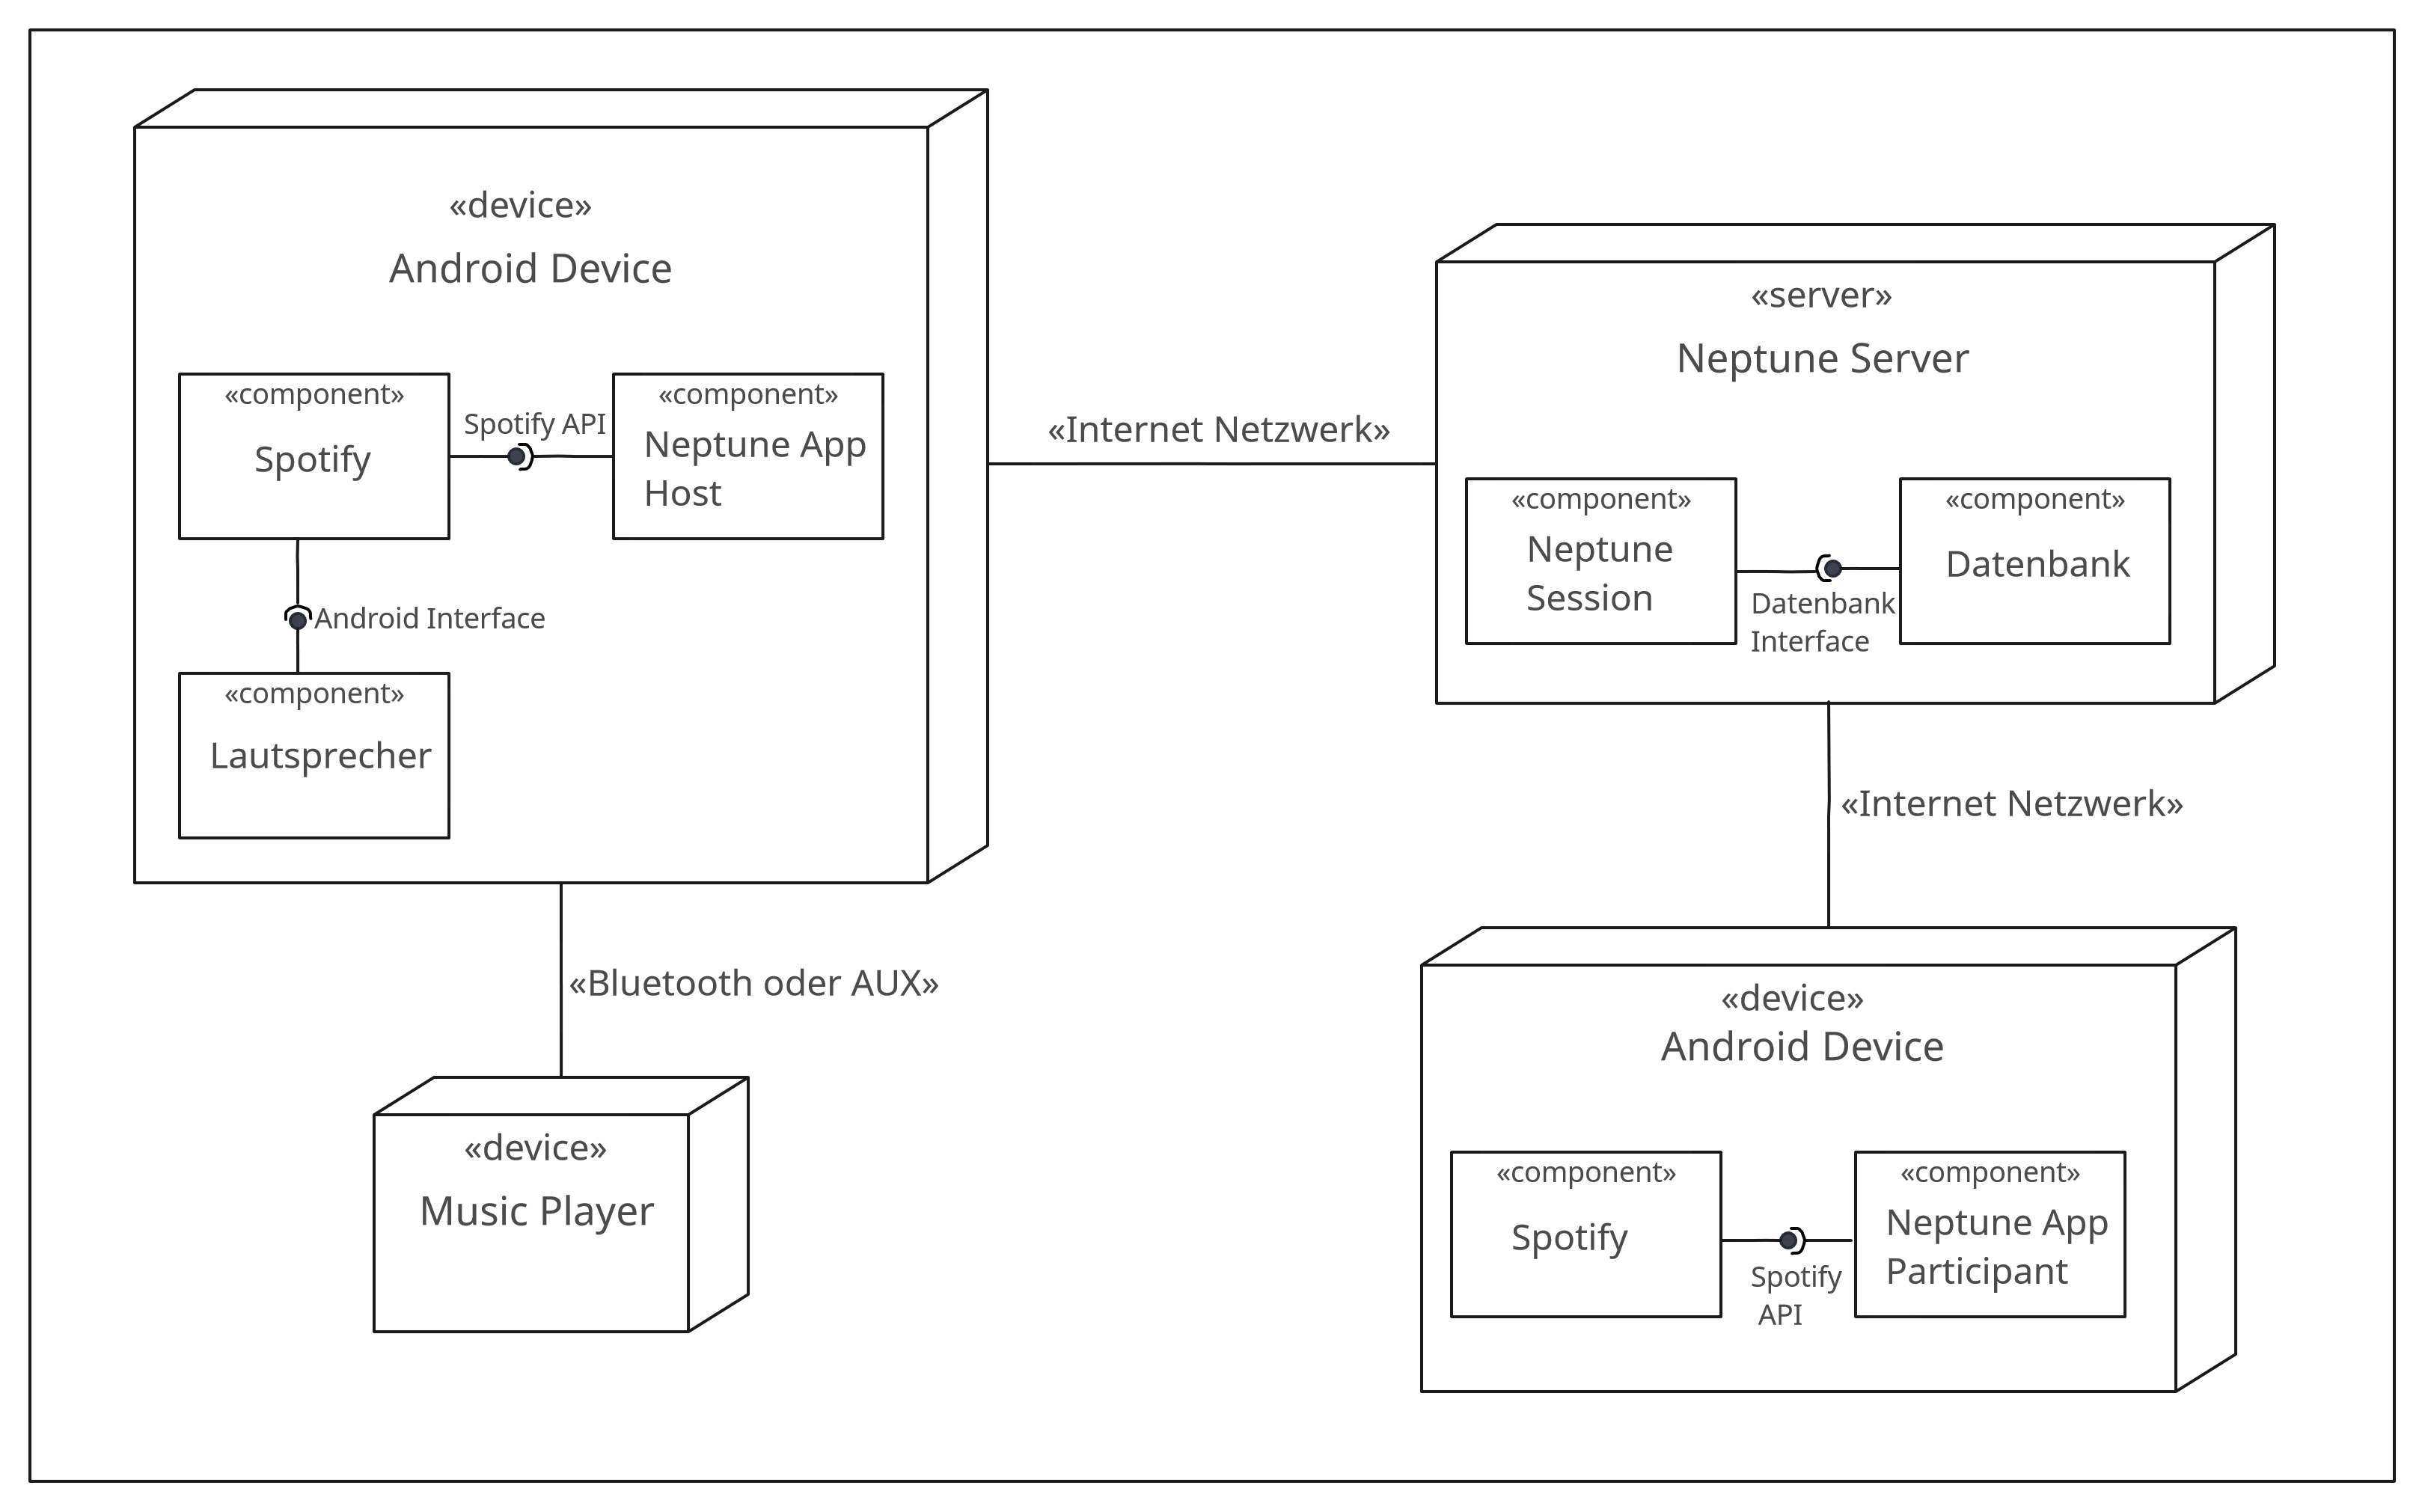
\includegraphics[width = 16cm]{LATEX/Pflichtenheft/GraphicDesigns/Verteilungsdiagramm.png}
    \caption{Verteilungsdiagramm}
    \label{fig:Verteilungsdiagramm}
\end{figure}



\chapter{Produktdaten}
\label{chap:Produktdaten}

\section{Systemdaten}
\label{sec:Produktdaten:Systemdaten}

Als Systemdaten werden sämtliche Daten zur Generierung der Benutzeroberfläche gespeichert, sowie die eindeutige Identifikation der App und Daten zum Auffinden des Servers. Zustandsdaten der App werden je nach Entwurfsentscheidung abgespeichert, um die App auch nach dem Schließen im selben Zustand erneut laden zu können. Es werden keine Benutzereinstellungen oder Historiendaten gespeichert. Auf dem Server werden Daten zum Zustand von Sessions gespeichert. Diese Session-Daten oder Teile von ihnen können auch kurzfristig lokal in der App der User gespeichert werden.

\section{Nutzerdaten}
\label{sec:Produktdaten:Nutzerdaten}

Es werden keinerlei sensiblen Nutzerdaten gespeichert. Im Fall des Musikdienstes Spotify müssen zur Verwendung der API keine Nutzerdaten gespeichert werden. Nur der generierte Nutzungstoken der API wird lokal gespeichert. Außerdem wird nach der Installation eine eindeutige Identifikation der App generiert, um User voneinander zu unterscheiden. Diese Identifikation wird lokal gespeichert und bei der Kommunikation von App und Server verwendet.



\chapter{Anforderungen an die App-Umgebung}
\label{chap:Appumgebung}

Wir stellen folgen Software und Hardware-Anforderungen an die App-Umgebung:

\begin{itemize}
    \item Als Gerät wird ein Smartphone oder gleichwertiges Gerät mit mindestens Android 7.0 benötigt.
    \item Eine jederzeit aktive Internetverbindung wird zur Nutzung der App-Funktionalität benötigt.
    \item Ein verknüpfter Spotify-Account wird benötigt, um als Full Participant an einer Session teilzunehmen.
    \item Ein verknüpfter Spotify-Premium-Account wird benötigt, um als Host eine Session zu erstellen und an ihr teilzunehmen.
\end{itemize}




\chapter{Tools und Ressourcen zur Entwicklung}
\label{chap:Entwicklungsumgebung}

\section{Software}
\label{sec:Entwicklungsumgebung:Software}

\begin{itemize}
    \item Entwicklung
    \begin{itemize}
        \item Android Studio Giraffe (Version 2022.3.1)
    \end{itemize}
    
    \item Versionsverwaltung
    \begin{itemize}
        \item Git
        \item GitHub (zur Kommunikation)
    \end{itemize}

    \item LATEX-Dokumente
    \begin{itemize}
        \item Overleaf
    \end{itemize}
    
\end{itemize}

\section{Hardware}
\label{sec:Entwicklungsumgebung:Hardware}

\begin{itemize}
    \item Gewöhnliche PCs und Laptops zum Entwickeln der App
    \item Verschiedene Android Smartphones mit mindestens Android 7.0 zum Ausführen und Testen der App
    \item Linux Rootserver
\end{itemize}



\chapter{Begriffserklärungen}
\label{chap:Begriffserklärungen}

\textbf{App}
 - Der Teil des Softwaresystems, der auf dem Android-Gerät des Nutzers läuft.

 \textbf{Full Participant}
 - Mit dem Musikdienst verknüpfter Participant, der Tracks im gesamten Katalog des Musikdienstes suchen kann.

\textbf{Host}
 - Ersteller einer Session, der (vorgeschlagene) Musik abspielt (kein Participant). Der Host benötigt ein Premium Abonnenment des Musikdienstes Spotify.

 \textbf{Musikdienst}
 - Der Musik-Streaminganbieter, über den die App Musik abspielt. Bei dieser App ist das Spotify.

 \textbf{Participant}
 - Teilnehmer einer Session (nicht der Host). Überbegriff für Full Participant und Restricted Participant.

 \textbf{Produkt}
 - Der Zustand, in dem das System nach Fertigstellung sein wird.

 \textbf{Queue}
 - Liste von Tracks, welche als nächstes durch den Musikdienst abgespielt werden.

 \textbf{Restricted Participant}
 - Nicht mit dem Musikdienst verknüpfter Participant, der nur Tracks von den bisher upgevoteten suchen kann.

 \textbf{Server}
 - Der Teil des Softwaresystems, der nicht auf dem Android-Gerät des Nutzers, sondern auf einem zentralen und externen Server läuft.

 \textbf{Session}
 - Eine Gruppe aus Participants und einem Host. In ihr können Tracks upgevotet und vom Host abgespielt werden.

\textbf{System}
 - Das gesamte zu entwickelnde Softwaresystem, Überbegriff von App und Server.

 \textbf{Track}
 - Lied bzw. Musikstück.

 \textbf{Upvote}
 - Bewertung auf einen Track. Je mehr Upvotes ein Track hat, desto beliebter ist er.

 \textbf{User}
 - Jeder Benutzer der App, Participant und Host sind User.

 \textbf{Vorschlagsliste}
 - Liste von Tracks einer Session, die mindestens ein Upvote haben. Ausgenommen ist der Playlist-Modus: In diesem ist die Vorschlagsliste gleichbedeutend mit der eingestellten Playlist.
 

\end{document}
